%\documentclass[12pt]{ociamthesis}  % default square logo 
\documentclass[12pt,beltcrest]{ociamthesis} % use old belt crest logo
%\documentclass[12pt,shieldcrest]{ociamthesis} % use older shield crest logo

%load any additional packages
\usepackage[all]{xy}
\usepackage[linesnumbered,lined,ruled]{algorithm2e}
\usepackage[font=sf, labelfont={sf,bf}, margin=1cm]{caption}
\usepackage{subcaption}
\usepackage{sectsty}
\allsectionsfont{\sffamily}

\title{Content and User Recommendation In Social Networks}
\author{Nathan Hale}
\college{Exeter College}

%\renewcommand{\submittedtext}{change the default text here if needed}
\degree{Master of Science}
\degreedate{Summer 2012}

%end the preamble and start the document
\begin{document}

%\nocite{*}

%this baselineskip gives sufficient line spacing for an examiner to easily
%markup the thesis with comments
\baselineskip=18pt plus1pt

%set the number of sectioning levels that get number and appear in the contents
\setcounter{secnumdepth}{3}
\setcounter{tocdepth}{2}


\maketitle                  % create a title page from the preamble info
%\include{dedication}        % include a dedication.tex file
%\include{acknowlegements}   % include an acknowledgements.tex file
\begin{abstract}

Social networking services have exploded in popularity over the past several years and the amount of content available on those services has grown correspondingly. With this much available content it is easy for users to be overwhelmed. Thus, it is in the interests of both the service operators and the users of such services to have access to effective methods for recommending novel content and users to connect with.

This dissertation proposes one such method, adapting and extending a method used in web search to the problem of recommending both users and content within social networks. It also demonstrates a novel (??) procedure for incorporating links that would otherwise render a social graph non-bipartite into a proper bipartite graph.

It is then demonstrated that this method is effective at recommending both content and users that a particular distinguished user may be interested in. This efficacy is demonstrated through both user evaluation and calculated metrics. A number of different variations to the methods are explored in order to refine the results further.

\end{abstract}


\begin{romanpages}          % start roman page numbering
\tableofcontents            % generate and include a table of contents
\listoffigures              % generate and include a list of figures
\end{romanpages}            % end roman page numbering

%now include the files of latex for each of the chapters etc

%Introduction
\chapter{Introduction}

\section{Motivation}

Over the past decade, a number of internet services dedicated to `social networking' have been created. These services allow people to share what they are doing with their friends and to see what their friends have done. They also frequently allow users to see the publicly shared content of other users who they find interesting, perhaps because they know them, perhaps because that person is a celebrity, or perhaps because that person consistently shares content that is interesting in some way such as breaking news, funny jokes, or interesting articles.

The popularity of these social networking services has grown tremendously over the past several years, and that growth has been accompanied by a corresponding growth in both the amount of content available on these networks and the number of services available. Facebook, the largest social network, had over 901 million monthly active users at the end of March 2012 and had over 125 billion friend connections between those users\footnote{http://newsroom.fb.com/content/default.aspx?NewsAreaId=22}. Twitter is another popular social network which has over 140 million active users as of May 2012, with more than 383 million users\footnote{http://www.guardian.co.uk/technology/2012/may/15/twitter-uk-users-10m} having created accounts at some point since the service was founded in 2006. Dozens of other smaller social networks have been created as well, aimed both at general audiences and niche audiences.

With this explosion of content and users it has become much more difficult for users to find novel content of interest to them and to find new users to connect with who might consistently produce such content. Because this may negatively impact the user experience it is in the best interests of both users and the operators of social networking services to provide methods to allow users to easily find interesting content and users.

Existing approaches to content and user recommendation (as described in Section~\ref{sec:ContentRecommendationResearch}) have focused on either a network-based approach, which examines the topology of the network and the connections between users, or a content-based approach, which seeks to take semantic and syntactic information from the content itself and use that to recommend other content. In many cases these approaches are still hamstrung by the same issues that vex individual users, namely the vast amount of data that exists in these social networks which can make analysing them a very difficult task.

Most social networks already provide some form of content recommendation to their users, usually in the form of a list of other users that they may know or be interested in which is created based on the connections that the user already has, i.e. a network-based approach. This is a step in the right direction, but it recommends only users, failing to recommend interesting individual pieces of content. On existing social networks where some content is recommended to users, content is usually only recommended in terms of what is popular amongst all users, without considering the individual user's own interests.

The purpose of this dissertation is to provide a novel and more effective method of recommending both users and content to users of social networking services despite the large amount of data involved. This dissertation will use a combination of a network-based approach and a content-based approach since both have been shown to have value. Taking both methods into account is also very helpful in making the process faster because it is possible to recommend both users and content while running only one algorithm.

In developing this method, it is hoped that such a technique could be put to use either directly by a social networking service or by a third party in order to improve the experience for their users by leading them to more interesting and relevant content. Furthermore, existing techniques for evaluating the effectiveness of such recommendations are very lacking, so it is hoped that new techniques can be used to improve the ability to evaluate both this scheme and future research in the field.

\section{Structure}

This dissertation is structured into six chapters, including this introduction describing the motivation behind the project and the problems it is intended to address.

Chapter 2 gives important background on what social networks are, with particular focus on features that most networks have in common. Two networks in particular, Facebook and Twitter, are discussed in depth to show how these generic features are implemented. This also provides insight on which of these features may be useful in recommending content and users. After giving this background information, existing research on social networks and content recommendation is examined as a means of seeing which network features might be useful for developing recommendations and what techniques have already been used.

Chapter 3 describes the general methodology used by this dissertation. The method is described without reference to any particular social network to emphasize that the technique being used can be applied to nearly any social network having the general features described in Chapter 2. The suitability of this method, known as the Co-HITS algorithm, to social network graphs is described, as are the methods used to transform the graph of the social network into a graph suitable for use by this algorithm.

Chapter 4 describes the specific implementation used by this dissertation. It describes how the data about the social network was selected and obtained and it describes how the challenges of the huge size of this data were dealt with. It then describes the implementation of creating the social graph and implementing the Co-HITS algorithm to run efficiently on this large graph.

Chapter 5 describes the results obtained using this method. Evaluating the results is not straightforward since there is not yet a canonical method of evaluating results in this research area. A number of techniques are proposed and the results of the algorithm for each evaluation technique are presented. Additionally, this chapter describes a number of modifications to the basic algorithm for recommendation and shows how each of these variations affects the results.

Chapter 6 concludes the dissertation. This chapter provides a discussion on how the performance of the specific method developed here could be improved and what future work could be done in this area to improve the overall method by modifying it more fundamentally. The dissertation ends with some concluding remarks on the method developed, its efficacy, and its suitability for real-world implementation.


% an explanation of the problem: a second chapter should explain the problem 
%to be studied, or the context in which the work takes place
\chapter{Background and Related Work}

This chapter begins by describing what social networks are and what features one can expect to find in them. In particular, the features of two of the largest social networks, Facebook and Twitter, are discussed in detail, including how those features might be useful in recommending novel content to users. Using this description for background, the discussion then moves to research that has already been done in this field and which techniques for content recommendation have shown promise so far.

\section{Social Networks}

Facebook and Twitter are certainly the most popular social networking services, with more than 1 billion user accounts between them. There are dozens of other social networks, however, including many with millions of users such as Google+, Pinterest, and LinkedIn. It would be impractical and of limited value to discuss the nuances of all of these services and to what degree they implement particular features, but some background is necessary in order to understand the work undertaken in this project. Because Twitter and Facebook are the most popular social networking services and demonstrate all of the common features of social networks this discussion will be limited to only these two services.

Before describing these two services and their features in detail, it is valuable to begin with a brief discussion of the general features that are common to all social networks. Examining these general features provides a good basis for comparison of how the general features are implemented by the two test cases. It is also helpful as a reference to show that while the study undertaken for this project was specific to one particular social networking service, the features used were actually quite generic and could easily be extended to other services.


\subsection{What are Social Networks?}

At its core, a social network is a set of users, a set of edges connecting those users, and content produced by those users. Depending on the network and the relationships between users, the edges may be either directed or non-directed, and sometimes a given network may include edges of both types. A non-directed edge indicates that both users are subscribed to each other's content while a directed edge from user A to user B indicates that while user A is subscribed to content produced by user B and will see all public content from user B, user B will not see any content from user A.

The types of content produced also vary depending on the network. Twitter famously limits content to 140 characters of text, a limit designed to ensure that it can fit within the standard text message size limit of 160 characters. Still, those 140 characters can contain links to any other sort of content, and as the service has developed various conventions have been created in an ad hoc manner by its users in order to mark up the text to provide additional meaning. Facebook users, meanwhile, can share much longer text updates, photos, links, and videos. 

Another common feature of social networks is the ability for users to create profiles to tell other users about themselves and to express their interests and desires. The importance of that profile depends on the network, and in some cases it is the primary form of content produced by users. LinkedIn, for example, is a social network designed for professional networking and job-seekers, and its user profile pages are essentially just extended CVs.

Social networks also frequently provide the ability for users to re-share or forward content from other users so that their connections can see that content. This allows links and pictures to make their way across the network and be seen by users who are not themselves connected to the original user who produced a piece of content. And, importantly for the task of recommending content, it provides a good insight into the types of content that the person re-sharing the content finds interesting.

The degree to which networks support these features varies widely, but most networks---and certainly the majority of the most popular networks---implement all of these features.

\subsection{Facebook}

Facebook was originally founded as a way for students at Harvard University to keep in contact with each other. Early versions of the website were rudimentary compared to the current behemoth---the only real features were the ability to become friends with other users and to fill out a profile indicating the user's birth date, home town, current location, interests, and similar biographical details. From those early beginnings the network expanded first to other universities and then to secondary schools before membership was eventually open to everyone.

As one of the oldest social networks which still enjoys a large user-base, Facebook has evolved quite a bit over the years since it was created. As other social networks have challenged it by introducing new features, Facebook has responded by adding versions of those same features with slight modifications to adapt them to the Facebook environment. Over the years of growth the modern version of Facebook has  slowly taken shape as features such as photo sharing, the news feed, and the `like button' have been introduced.

\subsubsection{Features}

The Facebook network is built around the concept of friends. The edges in the Facebook network are connections between users who (mostly) know each other in real life and are bi-directional. One user sends a friend request to a second user and if the second user accepts then the connection is created and each user can see content produced by the other.

Suppose that there is a user Alice who is friends with a user named Bob but not with a user named Carol. Bob, however is friends with Carol. Alice might share a piece of content $C_{A}$ with her friends, in which case Bob will see the update but Carol will not. Similarly, if Carol shares a piece of content $C_{C}$, Bob will see it but Alice will not. Finally, if Bob shares a piece of content $C_{B}$, both Alice and Carol will see it since both users are friends with Bob. This visibility is shown in Figure~\ref{fig:fb_content_visibility}.

\begin{figure}
  \centering
\begin{displaymath}
  \xymatrix{
    Alice \ar@<0.5ex>[r] & C_{A} \ar@{.>}@<0.5ex>[l] \ar@{.>}[dl] \\
    Bob \ar@{<-->}[u] \ar@{<-->}[d] \ar@<0.5ex>[r] & C_{B} \ar@{.>}@<0.5ex>[l] \ar@{.>}[ul] \ar@{.>}[dl]\\
    Carol \ar@<0.5ex>[r] & C_{C} \ar@{.>}@<0.5ex>[l] \ar@{.>}[lu] }
\end{displaymath} 
  \caption[Visibility of content on Facebook]{An example of how visibility of content works on Facebook. The dashed edges indicate the friendship connections between users. Directed edges from users to content indicate authorship, and dotted directed edges from content to users indicate which users can see that content.}
\label{fig:fb_content_visibility}
\end{figure}

The primary forms of content on Facebook are status updates, photographs, and links. Status updates are just text updates, sometimes telling other users what that person is doing, sometimes asking for advice, and sometimes just expressing emotions. Photographs and links are both self-explanatory, and are usually accompanied by captions or explanatory text from the user describing his or her thoughts on the content being shared. Each of these types of content is accompanied by a set of comments made by friends. Additionally, friends may 'like' the content by pressing the `like' button to indicate some sort of agreement, support, or genuine like of the associated status, link, or photograph without needing to leave a comment.

More recently, perhaps in response to competition from Twitter, Facebook has introduced the ability to share (forward) content from another user and to subscribe to public posts of another user or group, essentially creating a directed edge between those users. Returning to the example of Alice, Bob, and Carol, if Alice shares content $C_{A}$, Bob will see it but Carol will not since Alice and Bob are friends while Alice and Carol are not. Bob can re-share this, however (provided that Alice's privacy settings allow this) at which point Carol will be able to see it. This visibility relationship is shown in Figure~\ref{fig:fb_reshare}. Additionally suppose that Carol subscribes to the public updates of Alice. In this case, if Alice shares a photograph publicly, Carol will be able to see it without Bob having to re-share it since she subscribes to Alice's public updates. 

\begin{figure}
  \centering
  \begin{subfigure}[b]{0.3\textwidth}
    \centering
    \begin{displaymath}
    \xymatrix{
    Alice \ar@<0.5ex>[dr] &  \\
    Bob \ar@{<-->}[u] \ar@{<-->}[d]  & C_{A} \ar@{.>}@<0.5ex>[ul] \ar@{.>}[l] \\
    Carol  & }
    \end{displaymath}
    \caption{Before Bob reshares $C_{A}$}
    \label{fig:fb_reshare_before}

  \end{subfigure}
  \quad
  \begin{subfigure}[b]{0.3\textwidth}
    \centering
    \begin{displaymath}
    \xymatrix{
    Alice \ar@<0.5ex>[dr] &  \\
    Bob \ar@{<-->}[u] \ar@{<-->}[d] \ar@<0.5ex>[r] & C_{A} \ar@{.>}@<0.5ex>[ul] \ar@<0.5ex>@{.>}[l] \ar@{.>}[dl] \\
    Carol  & }
    \end{displaymath}
    \caption{After Bob reshares $C_{A}$}
    \label{fig:fb_reshare_after} 
  \end{subfigure}
  \caption[Visibility of reshared content on Facebook]{Visibility of content on Facebook before and after content is reshared. The dashed edges indicate the friendship connections between users. Solid edges between users and content indicate content authorship and resharing, and dotted edges between content and users indicate visibility. This figure does not include the situation where Alice subscribes to the public updates of Carol. }
  \label{fig:fb_reshare}
\end{figure}


As alluded to above, various privacy controls have been put in place over the years to give users control over who can see what content. Though the original idea of Facebook was that friends on Facebook would correspond to friends in real life, the actual mode of use didn't follow and people often found themselves in nominal `friendships' with acquaintances or people from different social circles with whom they didn't necessarily want to share all of their content. Thus, users can choose to share specific content only with specific sets of people and to restrict the re-sharing of their content. Additionally, users must decide whether posts will be public, visible only to friends, or visible only to specific friends.

Other popular features of Facebook allow users to create events and send invitations to their Facebook friends and the ability to run applications and games developed by third-party developers which leverage the user's social data to provide additional experiences.

\subsubsection{Content Recommendation}
\label{sec:FbContentRec}

Many of the basic features of Facebook would be very applicable for use in a content recommendation scheme. The basic edges between users present an obvious starting point, but other features could be leveraged to put a more accurate weight on edges between users. Users who frequently comment on one another's posts are more closely connected than users who never interact, for example.

Similarly, if a user likes a post or comments on it then it indicates that the content itself was relevant to that user, information which could be used to recommend future content of interest to that user. Attending common events would be another method of determining just how close two nominal 'friends' actually are---users who go to the same events in the real world are obviously much more likely to be good friends than users who do not.

The large amount of information on a Facebook user's profile is another piece of information that could be leveraged to recommend content. If two users declare similar interests on their user profile then it would be more likely that those users would be interested in content generated by one another.

Facebook itself has developed a system based on many of these components to help it recommend other users that it believes you may know and want to become friends with. One such project is described in \cite{Backstrom2010}.

The major drawback to studying content recommendation on Facebook is that the data is difficult to access. Most of the content created by users and the edges between those users are private and thus inaccessible to researchers. Therefore most studies focusing on Facebook, including that in \cite{Backstrom2010}, are undertaken at least in part by employees of Facebook participating in research and development to help advance the interests of the company.

The private nature of this data made it unsuitable for study in this dissertation, though many of the other components of the network would have provided a rich set of features to use in content recommendation. Facebook is discussed here to show that it has analogues to most of the major features of Twitter and that all of the research undertaken in this dissertation could easily be applied to Facebook if the data were available.

\subsection{Twitter}

\subsubsection{History}

Created in 2006, Twitter is a social network noted for the brevity of its content. The basic concept is simple: users provide status updates on what they are doing or thinking in up to 140 characters. The basic interface has changed very little since its inception and the feature set is still very similar to its beginnings, in marked contrast to the large number of features that are integrated into Facebook.

The original intent was that users could update their status and receive status updates from friends using SMS messages from their mobile phones, and thus the length of any given Twitter message was limited to be smaller than the maximum size of an SMS message, 160 characters.

The nature of the network began to change as smartphones---mobile phones capable of running applications and communicating with the internet---became ubiquitous following the release of Apple's first iPhone in 2007. Twitter provides an extensive Application Programming Interface (API) which has allowed application developers to create rich and visually pleasing interfaces to the service that have helped boost its popularity by making it even easier to use. As smartphones grew in popularity the need for and popularity of status updates via SMS faded, though the 140 character limit has remained.

Today, Twitter has over 140 million active users worldwide, and those users produce hundreds of millions of status updates each day. As a result, numerous attempts have been made to make sense of this vast source of public data about the feelings and activities of millions of people around the world. Research into this area is discussed in greater depth in Section~\ref{sec:InfoGatheringResearch}.

\subsubsection{Features}

Twitter updates are commonly known as \emph{tweets}, and the act of producing one is known as \emph{tweeting}. Within the research literature on Twitter, one person's \emph{Twitter feed}, the collection of all of the tweets that they have produced, is commonly called a microblog in reference to the previously mentioned 140 character limit imposed on each tweet. Edges between users are directed. If a user Alice follows a user named Bob but Bob does not follow Alice, Alice will see all of Bob's tweets, but Bob won't see any of Alice's tweets. This is shown in Figure~\ref{fig:twitter_content_visibility}.

\begin{figure}
  \centering
\begin{displaymath}
  \xymatrix{
    Alice \ar@<0.5ex>[r] \ar@{-->}[d] & C_{A} \ar@{.>}@<0.5ex>[l] \\
    Bob   \ar@<0.5ex>[r] & C_{B} \ar@{.>}@<0.5ex>[l] \ar@{.>}[ul] }
\end{displaymath} 
  \caption[Visibility of content on Twitter]{An example of how visibility of content works on Twitter. The dashed edge indicates that Alice follows Bob, but Bob does not follow Alice. The dotted edges represent who will see each piece of content in their Twitter stream. Note that Alice or Bob could always see the other users's content by visiting their Twitter feed, regardless of any follower/followee relationship between them.}
\label{fig:twitter_content_visibility}
\end{figure}

The terminology which will be used by this dissertation will be to refer to Alice as one of Bob's \emph{followers} and to refer to Bob as one of Alice's \emph{followees}. In contrast to Facebook, most tweets are visible to the public; the act of following Bob simply causes Bob's tweets to appear along with the tweets of Alice's other followees in Alice's \emph{Twitter stream}, which is the set of tweets of everyone that Alice follows. If Bob cared to see all of Alice's tweets he could simply visit her Twitter feed, which collects all of Alice's tweets.

Initially, this was the complete feature set of the service; it was possible to post updates and to subscribe to the updates of others. As Twitter became more popular its users began to develop a shorthand for indicating things to other users. As that shorthand became more codified many of these features were given native support by Twitter. The most important of these features are hashtags, mentions, and retweets.

Since the service only permits the sharing of text directly, it does not internally support sharing pictures, videos, or links. However, web addresses contained within the text of a tweet are highlighted and automatically turned into links, allowing pictures, videos, or any other content to be shared by hosting it externally and providing a link. A number of image hosting websites were developed specifically to support user uploads of photos which can then be linked from Twitter. The biggest issue with linking is that many web addresses are by themselves more than 140 characters, and even those which are not often would not leave much room for comment if included in their entirety. As a result, URL shortening services (such as bit.ly, t.co, and ow.ly), which take a complete URL and hash it down to 5 or 6 characters, have become popular. An example of such a link is seen in Figure~\ref{fig:retweet_hashtag}.

\paragraph{Hashtags}

Hashtags were created organically by users of Twitter\footnote{https://support.twitter.com/articles/49309-what-are-hashtags-symbols} as a way of tagging tweets on a similar topic. Thus, someone might tag a tweet about the University of Oxford by appending `\#oxford' to the message. Or, in keeping more with the brevity that is prized within tweets, they might integrate the hashtag into the message itself, something like `Currently visiting the University of \#Oxford'. Figure~\ref{fig:retweet_hashtag} contains a screenshot of a tweet which includes a hashtag.

Tagging tweets in this way clusters tweets which all discuss a particular topic and makes it easy to search. As this feature became widely adopted by users it was integrated to have native support by Twitter. Today, such hashtags appear as highlighted links within a tweet and clicking the link brings up other tweets that have used the same hashtag recently.

Twitter collects these hashtags and provides a list of topics that are currently popular amongst users. While these hashtags must not contain spaces or punctuation in order to be parsed properly, they are often stylized to contain entire phrases and questions to which users provide answers, such as \#MyFavouriteSongIs for discussing music. While certainly commonly used for banalities and idle chatter, these hashtags can also take on great importance for providing information during breaking news events. For example, during the Iranian political unrest of 2009, hashtags such as \#IranElections became popular for users in that country to disseminate information about protests \cite{Cha2010}.


\paragraph{Mentions and @replies}

Mentions are another important feature of Twitter, and like hashtags, they also started out as a convention amongst users before being adopted as a native feature by Twitter \cite{Java2007}. Mentions are simply a way of directing a tweet to the attention of a particular person. This is accomplished by pre-pending an @ symbol to their user name and including it in the tweet. Thus, to mention Bob, Alice would type `@bob' in her tweet. Mentions are collected by Twitter and can be seen even if the user being mentioned, henceforth referred to as the \emph{mentionee}, does not follow the mentioner. These mentions do not appear on a person's main Twitter feed, but are instead accessed from a special mentions page. If the username following the `@' character does not exist, the link is still highlighted but is not valid.


One distinction that is made is between an @reply and a mention. An @reply is the colloquial term given to mentions where the @username syntax appears at the beginning of the tweet as in the following sample tweet from Alice: ``@bob Hope to meet you after the presentation today!''. Because this is an @reply, this tweet would not show up in the main Twitter streams of Alice's followers (unless they also follow Bob). Since Bob doesn't follow Alice, this @reply also would not show up in his Twitter stream, only in his mentions. In contrast, a mention is a tweet that contains the @username syntax anywhere except at the beginning of the tweet, such as in this example tweet from Alice: ``Hoping to meet @bob after the presentation today!''. These tweets are visible on the Twitter streams of Alice's followers just like any other tweet, but are also collected for Bob along with all other tweets that mention him. Figure~\ref{fig:mention_reply} is a screenshot of a tweet which includes both a mention and an @reply.


\begin{figure}
  \centering
  
\includegraphics[width=1\textwidth]{mention_reply_example_figure}
  \caption[Example of a Twitter mention and @reply]{This tweet is an @reply to a user named `katiewardy' but also contains a mention of a user named `TeamGB', the official Twitter page for the United Kingdom's Olympic Team}
\label{fig:mention_reply}
\end{figure}



\paragraph{Retweets}

The final major feature of Twitter is yet another syntactic convention that was developed naturally by users and then given native support by Twitter: the retweet. A retweet is when a user repeats a tweet by another user to pass it along to their own followers, analogous to the re-sharing feature on Facebook. The common syntax is `RT @username [original tweet]', with the RT standing for retweet. The retweet is often sent along with a comment from the person retweeting about how they feel about what was said. While no specific convention exists for where to place this comment, two conventions often seen are to place a comment before the RT and to place it after the original tweet with some indication of the divide between the original tweet and the comment such as `//' or `...'. Figure~\ref{fig:retweet_hashtag} contains a screenshot of a tweet which includes a retweet which follows the convention of placing a comment before the RT.

\begin{figure}
  \centering
  
\includegraphics[width=1\textwidth]{retweet_hashtag_example_figure}
  \caption[Example of a Twitter retweet and hashtag]{An example of a Twitter retweet. Here, the resort has forwarded the positive tweet by user `eliseontravel' along with a comment of `We agree!' to their own followers. This tweet is also an example of a tweet containing a hashtag which was used in the original tweet: `\#Telluride'. The 'bit.ly/MUqOLf' at the end is a shortened link to an external website.}
\label{fig:retweet_hashtag}
\end{figure}


\subsubsection{Content Recommendation}

All of these features of the Twitter network are useful in content recommendation, and many of them have been used in existing studies as described in section~\ref{sec:ContentRecommendationResearch}. The primary advantage of the Twitter network as an object of study, however, is that the data is freely available and accompanied by an extensive API to allow the data to be queried and searched. This API has been used by numerous researchers to download large sets of tweets and the social graph accompanying it indicating which users follow which other users.

In fact, while studying Twitter it is actually a case of having far too much data to deal with easily than of not having enough data. Even though each tweet is no more than 140 characters, if the assumption is made that 100 million tweets are produced on a particular day (a very low estimate with today's usage), then that single day will contain roughly 14GB of data. Fortunately, previous researchers such as \cite{Kwak2010} and \cite{Choudhury2010} have already created some parsed versions of the data that can be used. More recently, a track of the Text Retrieval Conference (TREC)\footnote{http://trec.nist.gov/tracks.html} has been opened with regards to microblog research along with an enormous collection of tweets from 2011. Though these datasets are all extremely large and thus useful for research, they still represent only a small fraction of the total data present.

This vast amount of readily available data meant that Twitter was by far the best option to study in this project, even though most of the concepts would be simple to apply to other social networks if data were available for them since most of them have their major features in common with Twitter. As such, the remainder of this chapter will focus on Twitter since it is the object of study for this dissertation.


\section{Existing Research on Social Networks}

Twitter's simple and compact format and vast quantity of data has made it a popular target for research. The main topics of research are on the nature of the Twitter network itself, whether it is possible to gather useful information from Twitter, methods for determining what topics interest a particular Twitter user, and methods for ranking and recommending both tweets and users.

\subsection{The Twitter Network}

One of the earliest studies of the Twitter network was that of \cite{Java2007}, from 2007, only a few months after the service launched. The study was undertaken when Twitter had fewer than 100,000 users and during the two month study period only 1.3 million tweets were made. Clearly things have changed since this study, but it does still provide a number of interesting results. For example, they found that Twitter showed a high degree correlation---users with a large number of followers also tended to have a large number of followees. In the same vein, the distribution of indegree and outdegree had a similar power exponent to that of the web and the blogosphere.

The most important findings of \cite{Java2007} were the different categories of users and of content. They found that the content produced mostly fell into four different categories: daily chatter, conversations, sharing information, and reporting news. Importantly, conversation comprised nearly one-eighth of the tweets in their dataset. Presumably if a similar study were repeated today it would find a fifth content category: spam. Users were found to fall into three categories: information seekers, users who may tweet infrequently but still commonly check the site for the tweets of others; information sources, users who post information that others find valuable; and friends. At the time of the study friendship links constituted most of the links between users, though with more than 100 million users today, this is unlikely to be the case.

A later study by \cite{Cha2010} indirectly speaks to how much growth Twitter underwent between 2007 and 2010. At the time of that study in August 2009 Twitter had grown to nearly 54 million active users with 1.9 billion links between them and more than 1.7 billion tweets. The threshold for popularity investigated here, one million followers, is more than ten times greater than the total number of users in the 2007 study of \cite{Java2007}. \cite{Cha2010} found that while Twitter users with one million followers might seem intuitively to be the most influential, the number of followers alone was in general a poor measure of the influence that a user has.

\cite{Welch2011}, a 2011 study, investigated which links in the twitter network (e.g. follower links, retweet links, etc.) were most likely to preserve topical relevance. They found that the most important link type for preserving this topical relevance is retweet links. Crucially, they also found that ``traversing even a single follow link dramatically reduces the probability of topical relevance". In carrying out this study they repeated some of the experiments of \cite{Java2007} and found that most of the results from there still held true, despite the massive growth of the service.

A very important study for the purposes of this project is that of \cite{Kwak2010}, an in-depth examination of characteristics of the Twitter network. In many ways it is similar to the early 2007 study of \cite{Java2007}, but with a much more mature network. They studied things such as how likely a user was to reciprocate when someone followed them, the relationship between followee/follower numbers and number of tweets, the distribution of followee/follower numbers, the nature of trending topics, and the reasons behind and impacts of retweets, among other topics.

An important result from this study is that the number of followers/followees that users have behaves according to a strong power law with a long tail. There are hundreds of thousands of users with fewer than ten or twenty followers or followees, while only 40 users at the time of the study had more than one million followers. And of the users, 67\% were not followed by any of their followees! The results also showed that how many tweets a user had was a strong predictor of both how many followers and how many followees that person had, at least up to about 100 follower or followees.

Those results are interesting, but the crucial outcome of \cite{Kwak2010} for this project is the large dataset that was produced in order to find those results, of which the complete social graph (more than 1.2 billion edges) which was included and used for this project is the most important component. The social graph from this study was the main one used in the project, as discussed in Section~\ref{sec:SelectingADataset}.


\subsection{Gathering Information From Twitter}
\label{sec:InfoGatheringResearch}

Given the vast size of the Twitter network and the vast amount of data produced by its users in talking about what they are doing and how they feel, it is not surprising that studies have been undertaken to try to mine this data to gain more insight into what people believe and what they're discussing.

The study undertaken by \cite{O'Connor2010} attempted to predict the results of opinion polls based only on Twitter data. This process makes perfect sense when one considers that an opinion poll is really just an attempt to determine how a large population feels about something by sampling a small portion of that population and asking them how they feel. Analysing Twitter data, then, is akin to asking a much larger sample of that population.

Using a dataset of one billion tweets collected in 2008 and 2009, the research investigated three different possible opinion applications: election polls, job approval polls, and consumer confidence. For each application, tweets were analysed from a relevant period of time, such as in the run-up to the presidential election. For each tweet that contained certain trigger words that indicated relevance to a particular poll, the sentiment was analysed by simply seeing if a tweet had positive or negative words. All of the scores both positive and negative for a given period were summed and amalgamated and then compared to opinion polls from the same period of time.

The results were not perfect but did show a strong correlation for both job approval ratings and consumer confidence. Predicting election polling proved to be a more difficult task, and the correlation on those polls was not nearly as good. The strength of these results based on a very rudimentary method of sentiment analysis suggests that better techniques for analysing the tweets could improve the results.

A similar study was performed in \cite{Asur2010}, this time to try to predict the box office gross revenue of films. This study also reported some promising results from mining the sentiment of vast numbers of tweets in order to determine peoples' opinions.


\subsection{Determining User Interest}
\label{sec:UserInterestResearch}

A number of studies have focused on determining which topics are most often discussed by a user and which topics a user is most interested in reading about. The techniques from this area are very useful to the work undertaken in this project, particularly in determining the similarity of different pieces of content, e.g. as used in Section~\ref{sec:ProjectingToBipartite}. Section~\ref{sec:DeterminingContentSimilarity} describes the use of named-entity recognition (NER) for purposes of determining which tweets are related, but any of the techniques used in this section could be used instead, probably with better results, albeit at the expense of greater run times.

One study, \cite{Michelson2010}, used an ontology-based approach to determine a user's topics of interest. In this case, the ontology was the category structure of Wikipedia. For each tweet by a particular user, named entities were found using a named-entity recognizer. Those entities were then looked up in Wikipedia in order to disambiguate them and determine their categories. After repeating this process for all tweets by a user the process yields a pretty good set of the top ten topics of interest to that user.

A more mathematical approach was taken by \cite{Ramage2010}. They used a partially-supervised machine learning algorithm and achieved good results when categorizing the tweets. Their particular machine learning approach was Labelled Latent Dirichlet Allocation, which finds distributions of words which tend to occur in similar documents. These sets of similar words are taken to be the topics, and the topics of interest to particular users can determined by analysing their tweets for these words. The authors were unsure at the outset if this technique, commonly used for long documents such as news articles, would work for documents as short as tweets, and their results indicate that it is quite successful.

A more recent method, \cite{Pochampally2011}, attempted to determine the topics of interest for a particular distinguished user by finding which of their followees were most important and setting the topics discussed by those users as the topics of interest for the distinguished user. The study used an approach based primarily on the Twitter network, including follower/followee relationships and retweet/mention relationships in order to determine the list of top users. As in other studies, retweets were found to be the most reliable and were thus weighted the most heavily. Upon identifying the top users, they took an approach similar to that of \cite{Michelson2010}, using Wikipedia to look up terms and disambiguate them, though they used nouns returned from a part-of-speech tagger rather than named-entity recognition.


\subsection{Content and User Recommendation}
\label{sec:ContentRecommendationResearch}

Two main approaches exist in current research on recommending content and users, the network-based approach and the content-based approach. In the network-based approach, the connections between users and their interactions with one another via retweets and mentions form the primary basis for recommendation. In the content-based approach, meanwhile, the analysis is primarily focused on the tweets themselves, such as by determining which tweets are most similar to one another. The two approaches are by no means mutually exclusive and are often used in complementary ways.

The research described here shows that when recommending users and content, each approach has had some degree of success.

\subsubsection{Recommending Users}

\cite{Kwak2010}, the wide-ranging study that provided the dataset used for this project, included some analysis of potential network-based techniques for ranking users, though it was not the primary focus of the study. They used several techniques: ranking users in terms of number of followers, running the PageRank algorithm on the social graph, and ranking users in terms of how many times their content had been retweeted. As expected based on the results of \cite{Welch2011}, the number of retweets was the best of these ranking schemes. PageRank and the number of followers metric produced nearly identical results, suggesting based on the results of \cite{Cha2010}---namely that a user's number of followers is a poor measure of their influence---that PageRank is not a good technique to use for recommending users. The PageRank algorithm was originally developed by Google for web search and is well suited for that application. Applying it to the social graph seems promising intuitively, which is perhaps why it has been investigated a number of times, but the results suggest that it is not well suited to the task of user recommendation.

Still, PageRank has been used by other studies, such as in \cite{Weng2010}. They called their method TwitterRank because it differed slightly from original PageRank. Rather than visiting all users with uniform probability over links as in the random walk of PageRank, TwitterRank performs a topic-specific random walk using topics derived using Latent Dirichlet Allocation. Their results indicate that this modification allowed TwitterRank to outperform both the PageRank metric and a metric based on the indegree of nodes when ranking tweets. The performance improvement over page rank was small, however.

A hybrid approach utilizing both network and content information was taken by \cite{Armentano2011}. The goal of the research was to provide user recommendations in some sort of a ranked order. A network based approach was taken first in order to  discover potentially interesting users. From that unordered list of potentially interesting users a ranked list is created by comparing the users based on the content that they produce to a reference document of what the user is interested in. Two strategies specifically used for building the user profile are the user's own tweets and the tweets of the user's followees.

Another piece of work focused on recommending users is presented in \cite{Hannon2010}, which recommends users based purely on content. As with a number of other approaches, the major choice explored is what to use as the reference content to which other users are compared. Several different strategies are compared, some of them overlapping with those examined by \cite{Armentano2011}. The tweets of the user, their followees, and their followers were all considered, as were the lists of users' followers and followees. Additionally, combinations of these methods were employed in a hybridized approach. For each means of building them, the user profile documents were compared as TF-IDF valued word vectors (see Section~\ref{sec:ContentScoringMethod} for more details on TF-IDF weighting). The hybrid approaches performed the best, generally speaking. 

\subsubsection{Recommending Content}

Attempts to rank individual tweets have also been made, such as in \cite{Duan2010}, which used a content-based approach to this recommendation. Here, various content features are gathered for each tweet and then a learning algorithm is employed to evaluate which of these features should be ranked most highly. The various features that were evaluated can be divided into three basic groups: those based on the content of the tweets themselves, those based on Twitter-specific features, and those based on the authority of the users who created the tweet.

The features for the content of the tweets were represented by the Okapi BM25 or cosine similarity score between a tweet and a query being evaluated. The twitter-specific group included features such as the length of the tweet, whether it contained hashtags, whether it contained a URL, and how many times it had been retweeted. Finally, the account authority group included metrics such as how many followers the author of the tweet has and their PageRank score within the twitter network. Surprisingly, the mere presence of a URL was found to be the most important feature, and the length of the tweet was also found to be very predictive.

\subsubsection{Recommending Both Users And Content}

The work of \cite{Kim2011} used a machine learning algorithm to recommend both users and specific content in a system that they called TWITOBI. The approach is primarily based on the content of tweets, but some information about who follows whom in the network is utilized. A probabilistic model based on the expectation maximization algorithm is trained to properly rank both tweets and users via a similar technique. 

The sample size in terms of number of users was fairly small, consisting of only 8,405 users, but the sample size in terms of number of tweets was very large, with more than 12 million tweets by those 8,405 users. No discussion of how those users were decided upon is included, which when combined with the small number of users makes some of the results a bit suspect.

\subsubsection{Common Threads}

Many of the methods for recommending users and content utilize similar ideas in making their recommendations. The literature indicates via multiple studies that retweets are a very important predictor of what a user is interested in and that retweets are also an excellent indicator of how much influence a user has over others. It is also clear from existing research that the PageRank algorithm, while useful to some degree, does not perform very well at predicting which users will be most influential on a given user.

Most recent research has not focused specifically on either the network-based approach or the content-based approach, preferring instead to take useful features from each. This dissertation takes the same tack, utilizing useful features from both the network and the content. In many cases, features used successfully in the research reviewed here were not used for various reasons, but would make excellent additions to the methodology and implementation described in chapters 3 and 4.






%3 -- Method
\chapter{Methodology}

This chapter describes the methodology used in this dissertation to recommend both content and users to a particular user referred to here as the \emph{distinguished user}. Items are recommended based on both the social network structure surrounding the distinguished user and on the actual content produced by the distinguished user and by others in the surrounding network.

The various aspects of the method are intentionally described as generally as possible and without reference to any particular social network. This generality is important because while the experiments described in Chapter 4 and Chapter 5 are specific to Twitter, the methodology described here could just as easily be applied to Facebook, Google+, or many other social networks.

\section{Simple Approach}

The nature of a social network---a group of users connected to one another by various relationships---suggests that creating a graph is the best way to analyse the network. There are many algorithms suitable for the task of analysing such a graph and much research has gone into applying these algorithms to Twitter and other social networks. Additionally, research has been done to analyse the nature of social graphs to determine things such as the average degree of nodes (i.e. users) in the network and the average distance between nodes. This research was discussed at length in the previous chapter.

\begin{figure}
  \centering
\begin{displaymath}
  \xymatrix{
    A \ar[dr] \ar[dd] &  \\
      & B \ar[dl] \\
    C \ar[ur] & }
\end{displaymath} 
  \caption[Simple graph of a social network]{A simple graph of a social network containing three users. User A follows user C, user A and user C both follow user B, and user B follows only user C. }
\label{fig:simple_social_network_graph}
\end{figure}

The obvious approach to take is to build a graph where each user is a vertex and the relationships between those users are the edges, as in Figure~\ref{fig:simple_social_network_graph}. Thus, if user A follows user B then there will be a directed edge from vertex A to vertex B. When using the network-based approach for recommendation, this basic graph of the social network is often used, e.g. as in \cite{Hangal2010}. If it is desirable for the analysis to take the meaning of the content into account then this basic graph can be extended by creating edges between users who frequently discuss similar topics. This can be extended further by weighting the edges based on the strength of the relationship as determined by factors such as common activity as described in Section~\ref{sec:FbContentRec}. \cite{Hangal2010}, for example, augmented the basic social graph with additional links based on influence calculations.

Once a weighted graph such as this has been constructed a number of different algorithms can be employed including random walks, as in \cite{Backstrom2010}, the PageRank algorithm, as in \cite{Weng2010}, or simply searching for the strongest links to users who are not already connected to the distinguished user.

The obvious limitation to this simple approach is that it has no way of recommending particular pieces of content---the best it can hope to do is to select content from the top users using some similarity metric to compare that content to content that the user has already indicated interest in. Since the goal of this dissertation is to recommend both users and content this simple approach is clearly not sufficient.

\section{Co-HITS}

\subsection{Background and Suitability}
\label{sec:CoHitsBackground}

Deng et. al. \cite{Deng2009} developed an algorithm that they dubbed Co-HITS to use for ranking web queries and documents. The name of this algorithm is in reference to the famous HITS algorithm \cite{Kleinberg1999} for ranking websites. Co-HITS is similar to HITS, and in fact with particular values of the personalized parameters (see Section~\ref{sec:CoHitsParameters}) the algorithm reduces to the standard HITS algorithm. As with normal HITS, Co-HITS is an online algorithm, meaning that scores must be obtained for each unique query at query time rather than calculating the score once and then storing the results.

Two major differences between Co-HITS and HITS are the introduction of an initial score and that Co-HITS is designed to operate on a bipartite graph. The initial score factor is particularly important because it makes it possible to include content information in the algorithm by initializing scores based on content similarity. Co-HITS also does away with the concept of differing scores for hubs and authorities, instead keeping only one score.

The obvious objection to using this algorithm for recommending users and content is that the graph of a social network as in Figure~\ref{fig:simple_social_network_graph} isn't bipartite at all. However, the two classes described by \cite{Deng2009}, search queries and web documents, can be adapted to the task of content and user recommendation by reformulating the social network graph not with users as vertices and connections between users as edges, but with both users and content as vertices and with edges between user vertices and the vertices representing content produced by that user rather than between users.

\begin{figure}
  \centering
\begin{displaymath}
  \xymatrix{
    A \ar@{<->}[r] \ar@{<->}[dr] & C_{A_{1}} \\
      &  C_{A_{2}} \\
    B \ar@{<->}[r] & C_{B} \\
    C \ar@{<->}[r] & C_{C} }
\end{displaymath} 
  \caption[Simple bipartite graph of a social network]{This simple bipartite version of the graph of a social network shows how a social network can be made to be bipartite by incorporating generated content into the graph and creating edges between users and the content generated by those users. This also demonstrates that this process alone is not enough to provide a useful graph since this graph is very disconnected.}
\label{fig:disconnected_bipartite_graph}
\end{figure}

This new formulation of the social graph is clearly bipartite, as demonstrated in Figure ~\ref{fig:disconnected_bipartite_graph}, making the Co-HITS algorithm applicable to it. Unfortunately it is also clearly a very disconnected graph since users are only connected to the content that they produce, leaving no connections to other users or other content. This is addressed in section~\ref{sec:ProjectingToBipartite}; for now it is enough that this graph is bipartite and thus that the Co-HITS algorithm can be applied to it.


\subsection{Algorithm}
\label{sec:CoHitsAlgorithm}

This section contains a summary of the Co-HITS algorithm as described in \cite{Deng2009} but applied to the case of ranking users and content in social networks rather than ranking web queries. Some of the variable names have been changed from that paper's notation to make it more clear what the variables refer to in the context of social networks.

Let the set of all content be called $T$ and each member of that set be called $t$. Similarly, let the set of all users be called $U$ and each member of that set be called $u$. Then let the probability of transitioning from a particular user $u_{i}$ to a particular piece of content $t_{j}$ be denoted as $w_{ij}^{ut}$ and the probability of transitioning from content $t_{j}$ to user $u_{i}$ be denoted as $w_{ji}^{tu}$. The initial score (discussed in section~\ref{sec:InitializationOfScores}) for a given user node and content node will be indicated as $u_{i}^{0}$ and $t_{k}^0$, respectively. In both cases the initial scores are normalised such that $\sum\limits_{k \in T} t_{k}^{0} = 1$ and $\sum\limits_{i \in U} u_{i}^{0} = 1$. Given these definitions, the generalized Co-HITS equations are given in \cite{Deng2009} as follows:

\begin{center}
\[u_{i} = (1 - \lambda_{u}) u_{i}^{0} + \lambda_{u}  \sum\limits_ {k \in T} w_{ki}^{tu} u_{k}\]
\[t_{k} = (1 - \lambda_{t}) t_{k}^{0} + \lambda_{t}  \sum\limits_ {j \in U} w_{jk}^{ut} x_{j}\]
\end{center}

The paper goes on to describe further refinements under the assumption that only one set of vertices is desired to be scored. However, the goal for this project is to score both sets of vertices, so that refinement, consisting of substituting one equation into the other, will not be discussed. Note that the personalized parameters $\lambda_{t}$ and $\lambda_{u}$ will be discussed in Section~\ref{sec:CoHitsParameters}.

From these general Co-HITS equations, \cite{Deng2009} describes two frameworks to arrive at final scores for each node in the graph, the iterative framework and the regularization framework. The approaches are similar to the multiple approaches to determining PageRank in that one involves iteration and propagation of scores while the other involves matrix operations and more intense computation.

As the name implies, the iterative framework involves iteratively propagating the scores between the nodes using the above equations until achieving convergence. The paper states that their empirical results assert that convergence usually occurs within approximately ten iterations. Experiments done for this project and discussed in Chapter 4 indicate that this is accurate. The initial scores are normalised so that the scores for each set $T$ and $U$ sum to one. A convenient consequence of the above equations is that after each iteration of the algorithm the sums each of each set, $\sum\limits_{k \in T} t_{k}$ and $\sum\limits_{i \in U} u_{i}$, will still sum to one without need for an additional normalisation step.

The regularization framework, meanwhile, involves transforming the transition probabilities into a transition matrix and using that matrix along with some other derived equations to solve for the final results directly. The final step of this calculation involves a matrix inversion. As described in the paper, this operation can be done efficiently provided that the matrix is sparse and small. That works well for the test case described in \cite{Deng2009}, because their graph is indeed very sparse as well as being quite small (only 50,000 entries). This method is not well suited for a social network after application of the projection procedure described in section~\ref{sec:ProjectingToBipartite} because this graph is quite dense and extremely large since millions of pieces of content are produced each day, making the calculation computationally much more difficult and this framework less tractable than the iterative framework.


\subsection{Parameters}
\label{sec:CoHitsParameters}

The Co-HITS equations described above each include a so-called personalisation parameter $\lambda \in [0,1]$, which determines how much weight the initial score has on the final outcome. The closer a given $\lambda$ parameter is to 0, the more weight the initial score is given in calculating the score after each iteration.

Setting both $\lambda$ parameters to 0 simply means that the final score will be equal to the initial score. Setting both $\lambda$ parameters to 1, meanwhile, makes the algorithm into something much more akin to the standard HITS algorithm---the scores of each vertex are determined entirely by the scores of the nodes transitioning into that vertex. If only one of the $\lambda$ values is set to 0 then the algorithm will converge after only one iteration once the scores of the corresponding set of the bipartite graph have been propagated across to the other set. Finally, \cite{Deng2009} indicates that if only one of the $\lambda$ values is set to 1 then the algorithm becomes something akin to the Personal PageRank algorithm\footnote{The Personal PageRank algorithm is an extension of the PageRank algorithm which takes the preferences of the user regarding what type of content they wish to see into account when performing the random walk of the graph.}

Conceptually it makes sense to set the $\lambda$ parameters according to the confidence in the initial scores. If they are believed to be quite accurate for one or both sets of vertices in the bipartite graph then more weight should be placed on the initial score by moving the $\lambda$ value closer to 0. If, on the other hand, very little is known about the accuracy or values of the initial scores for a particular set of vertices then the $\lambda$ value should be closer to 1.

For the particular data set used in \cite{Deng2009}, $\lambda$ values of 0.7 and 0.4 were found to have particularly good results. Chapter 4 of this dissertation has more information on the values that were found to have good results for the social networking dataset used here.

\section{Projecting to a Bipartite Graph}
\label{sec:ProjectingToBipartite}

One of the key insights of this project was how to transform the social graph of a social network, which is very clearly not a bipartite graph, into a bipartite graph suitable for use with the Co-HITS algorithm or other algorithms specific to bipartite graphs such as \cite{Kunegis2010}. Section~\ref{sec:CoHitsBackground} has already described how a social network can be made into a simple bipartite graph by taking users and content as vertices and connecting users to the content which they produced.

Unfortunately, this basic process leaves a very disconnected graph and discards all of the network information about which users are connected to which other users, which is a very important piece of information. It also ignores the connections between pieces of content, such as whether they are forwards of a particular piece of content and whether they discuss similar topics to other pieces of content.

This information can be recovered by projecting the network connections between users so that they are represented by connections between user vertices and content vertices. If a user Alice is connected to a user named Bob and a user named Carol in the social graph (as in Figure ~\ref{fig:before_network_projection}), then this projection would connect content $C_{A}$ produced by Alice to both Bob and Carol in the output bipartite graph, Figure~\ref{fig:after_network_projection}. This process makes sense intuitively because it is clear that if Bob and Carol see this content---which they probably will, given their connection to Alice---then it is exerting some influence on them.

\begin{figure}
  \centering
  \begin{subfigure}[b]{0.4\textwidth}
    \centering
    \begin{displaymath}
    \xymatrix{
    Alice \ar@{<->}[r]  & C_{A} \\
    Bob \ar@{<->}[r] \ar@{-->}[u]    & C_{B} \\
    Carol  \ar@{<->}[r] \ar@{-->}@/^2pc/[uu] & C_{C} }
    \end{displaymath}
    \caption{Before projection}
    \label{fig:before_network_projection}

  \end{subfigure}
  \quad
  \begin{subfigure}[b]{0.4\textwidth}
    \centering
    \begin{displaymath}
    \xymatrix{
    Alice \ar@{<->}[r]  & C_{A} \\
    Bob \ar@{<->}[r] \ar@{<->}[ur]    & C_{B} \\
    Carol  \ar@{<->}[r] \ar@{<->}[uur] & C_{C} }
    \end{displaymath}
    \caption{After projection}
    \label{fig:after_network_projection} 
  \end{subfigure}
  \caption[Projecting network connections into the bipartite graph]{ Demonstration of projecting network connections, indicated in (a) by the dashed lines, to make the graph bipartite and more connected. }
  \label{fig:network_projection}
\end{figure}

Besides the obvious and explicit connections between users in a normal social network there are also implicit connections between the individual pieces of content that those users create. For example, in the case of Twitter, two tweets which include the same hashtag (e.g. \#Oxford) have an implicit connection, as in Figure~\ref{fig:before_content_projection}. The projection procedure can easily be extended to apply to content by connecting users who have produced content to all of the other pieces of content which are linked to their own. Thus if Bob mentioned \#Oxford in a piece of content, he would be connected to all other content in the graph which also mentioned \#Oxford, as indicated in Figure~\ref{fig:after_content_projection}.

\begin{figure}
  \centering
  \begin{subfigure}[b]{0.3\textwidth}
    \centering
    \begin{displaymath}
    \xymatrix{
    Alice \ar@{<->}[r]  & C_{A}   \\
    Bob \ar@{<->}[r]    & C_{B}   \\
     & \\
    Carol  \ar@{<->}[r] & C_{C} \ar@{<-->}[uu]|{\#Oxford}  }
    \end{displaymath}
    \caption{Before projection}
    \label{fig:before_content_projection}

  \end{subfigure}
  \quad
  \begin{subfigure}[b]{0.3\textwidth}
    \centering
    \begin{displaymath}
    \xymatrix{
    Alice \ar@{<->}[r]  & C_{A}   \\
    Bob \ar@{<->}[r]    & C_{B}  \ar@{<->}[dl] \\
    Carol \ar@{<->}[r] & C_{C} \ar@{<->}[ul]  }
    \end{displaymath}
    \caption{After projection}
    \label{fig:after_content_projection} 
  \end{subfigure}
  \caption[Projecting content connections into the bipartite graph]{ Demonstration of projecting connections between related pieces of content, indicated in (a) by the dashed lines, to increase the connectivity of the bipartite graph. }
  \label{fig:content_projection}
\end{figure}

This projection also makes sense because if Alice creates a piece of content then she is likely to be interested in other content which is related to it. This process of projecting the content links isn't limited to just hashtags. Any two pieces of content determined to be similar could have their implicit links projected in the same way. That could mean that they both mention similar named entities, that it can be determined that they discuss the same topic, that they link to the same external web address, or any number of other means of determining the similarity of two pieces of content.

A number of other projections can be made to add other features of the social network to the bipartite graph. For example, \cite{Welch2011} reveals that in Twitter retweets are one of the most important indicators of what is interesting to a user. Retweets---or more generally, re-shares of the content of others---can be included in the bipartite graph in a number of ways such as by strengthening the weight of edges connecting the sharer to the content of the original author, by connecting the content produced by the original content author's connections to the sharer, or by connecting the content produced by the original content author to the connections of the sharer.

Projecting out the links between users and the links between content makes the bipartite graph much more connected and also models the real-world influence that particular network characteristics exert. Depending on the test being run, some or all of these edges may be directed rather than undirected and they may be weighted or not. Some analysis of those design decisions is presented in Chapter 4.


\section{Method for Initializing Scores}
\label{sec:InitializationOfScores}

A key factor in the accuracy of the final scores when using the Co-HITS algorithm is the initial scores provided for each set of vertices. How much of an effect the initial scores have is dependent on the $\lambda$ parameters, but unless both are set to 1 the initial scores will still have a major impact on the final results. It is therefore quite important to choose a good method for determining those initial scores. In the absence of any known metric for determining the scores it is necessary to set the initial scores for a particular set to a uniform value, which indicates that all of them are equally likely to be relevant at the outset.

Fortunately, in social networks, it is possible to make some very accurate initial determinations about content and users which may be relevant.

\subsection{User Scores}
\label{sec:InitializationOfUserScores}

Much work has been done on the so-called link prediction problem which seeks to predict which links will be created between users in a social network, i.e. which other users are most relevant to a given user. \cite{LibenNowell2007}, \cite{Kunegis2010}, and \cite{Backstrom2010} are all examples of studies that have been done on this subject.

Because this process of determining original scores is only the initial step in the recommendations, for this project it makes sense to choose a method which is as fast as possible while still maintaining a high degree of accuracy. \cite{LibenNowell2007} studies a number of different methods of link-prediction, ranging from very fast and easy to calculate to very complex calculations. Fortunately, one of the most accurate methods is also one of the easiest to calculate, which is the method of Adamic and Adar from \cite{Adamic2003}.

If $\Gamma (x)$ is defined as the set of all connections (neighbours) of vertex $x$, then the similarity score for two users x and y is given as: 

\begin{center}
\[
\sum\nolimits_{z \in \Gamma (x) \cap \Gamma (y)} \frac{1}{\log |\Gamma (z) |}
\]
\end{center}

The initial score for all of the user vertices in the bipartite graph can be computed by iterating through all of the users and comparing them to the distinguished user with this metric. This function handily penalizes the effect that more popular users have on the scores by virtue of appearing more frequently while weighting less popular users more highly.

Depending on which particular social network is being examined, it may make sense to use slightly different versions of the $\Gamma$ function. For example, in Facebook it might make sense to consider only the neighbourhood of close connections, while in Twitter it might make sense to find the intersection of the followees of the distinguished user and the followers of the user being scored rather than the intersection of the followers of both.

Both the simple common neighbours function, given by:
\begin{center}
$| \Gamma (x) \cap \Gamma (y) |$
\end{center}

\noindent
and the Jacard Coefficient, given by:

\begin{center}
\[
\frac{| \Gamma (x) \cap \Gamma (y) |}{| \Gamma (x) \cup \Gamma (y) |}
\]
\end{center}

\noindent
were found by \cite{LibenNowell2007} to present good results as well and could be used in cases where a more lightweight function is desired.

\subsection{Content Scores}
\label{sec:ContentScoringMethod}

Much research has also been done on comparing the similarity of content, usually in the form of document similarity. Such algorithms can be a straightforward comparison of the number of words which overlap in the two pieces of content or they can be much more complex and use ontologies or other methods of deriving semantic meaning to compare the two pieces of content.

As with the initial user scores, it is desirable that the initial content scores be fast and easy to compute. A natural choice is the cosine similarity metric, which is both very common and very easy to compute. This metric requires that the pieces of content (referred to as documents in the remainder of this section) be represented as vectors in the standard term frequency--inverse document frequency (tf-idf) form.

In this form, the documents are represented as vectors where each dimension corresponds to a different term that appears somewhere in one of the documents in the collection. The value of each dimension is the tf-idf value. In its most common form, the tf-idf value for a given term is computed as:

\begin{center}
\[
tf(t) \times idf(t) = |t| \times \log(\frac{|D|}{df(t)})
\]
\end{center}
\noindent
where $tf(t)$ is the frequency of term $t$ within the document in question (represented above by $|t|$), and $idf(t)$ is the inverse document frequency for that term, which is found by dividing the number of documents in the collection (represented above as $|D|$) by the number of documents in the collection which containing term $t$ (represented as $df(t)$). The denominator of the idf function can lead to a division by zero if a term does not appear in the collection, so either that needs to be detected and the corresponding tf-idf value set to zero or each df(t) values should be incremented by one.

Once tf-idf vectors have been created for both of the documents $\hat{a}$ and $\hat{b}$ being scored, the cosine similarity metric itself can be computed as:

\begin{center}
\[
\frac{\hat{a} \cdot \hat{b}}
        {|\hat{a}| |\hat{b}|} 
=
\frac{ \sum\nolimits_{i} a_{i} b_{i} }
       { \sqrt{\sum\nolimits_{i} (a_{i})^{2} } \sqrt{\sum\nolimits_{i} (b_{i})^{2}} }
\]
\end{center}

This equation for the similarity between two vectors lies in the range $[-1,1]$ in the general case. However for document vectors the individual terms can never be negative and so the range of the similarity lies in the range $[0,1]$.

For actually computing the initial scores of the bipartite graph it is necessary only to iterate through all of the pieces of content and compare each one to a reference document using the cosine similarity metric. The only remaining question, then, is the choice of the reference document which best indicates which documents will be relevant. Based on \cite{Welch2011}, the best option would likely be the set of content which the distinguished user has re-shared, since that is the best indicator of the type of content that user would like to see. If that set is empty, then some secondary choices might be the set of all documents produced by connections of the distinguished user or the set of all documents produced by the distinguished user.

While the scores produced by this method are not as accurate as the methods for initialising user scores discussed in Section~\ref{sec:InitializationOfUserScores}, the resulting scores are still quite reasonable and the scoring process is very fast. Plus, tf-idf scoring and cosine similarity are very widely used methods and are supported by a wide range of tools and libraries. The fact that the initial scores produced for the content are not quite as accurate as those for users can be dealt with by simply moving the value of the $\lambda_{t}$ parameter closer to 1, dampening the impact of the initial score.


%4 -- Implementation


\chapter{Implementation}

This chapter describes how the method of Chapter 3 was actually implemented for this project, a non-trivial step considering the major difficulties associated with the vast amount of data used. This includes discussion of the way in which some of the parameters of the methodology were instantiated in addition to the specific implementation details for this project. It begins by describing how the dataset was selected and the challenges that the large dataset presented in terms of storing and accessing the data. From there it moves on to describe how the bipartite graph was constructed, including selection of tweets and users, construction of edges,  and initialization of scores. From there, the actual implementation of the algorithm is described both in words and in pseudocode before finally describing the method of retrieving the results from the database.

Java was chosen as the programming language for this project due to the wide adoption of libraries available to interface with it and the ease of development with those libraries. The Lucene information retrieval library\footnote{http://lucene.apache.org/core/}, for example, is originally written in Java and was used to index the tweets in a way that made tf-idf cosine-similarity calculations easy. It also facilitated easy search of the tweet database which was useful during the development process to learn more about the nature of the dataset. In addition to Lucene, the Java Database Connectivity library (JDBC) was used to interact with the PostgreSQL database and the Stanford named-entity recognizer was used for the named entity recognition.

\section{Selecting a Dataset}
\label{sec:SelectingADataset}

When beginning the project, one of the first questions was which dataset to use. There were four possibilities: downloading data via the Twitter API specifically for this project, the Choudhury data set (\cite{Choudhury2010}), the Stanford data set (\cite{Yang2011}) using the social graph of Kwak et. al. (\cite{Kwak2010}), and the database created for the Text Retrieval Conference (TREC). Each had advantages and disadvantages.

Given the availability of existing datasets that would meet the needs of the project, the possibility of downloading a social graph and set of tweets specifically for this project was dismissed early on, leaving the task as one of selecting which of the three datasets was best.

The smallest dataset was the Choudhury data. It consisted of tweets collected between late 2008 and late 2009 and contained more than 10 million tweets and more than 800,000 edges. This database is much smaller than the network was at the time it was created; it contains a tiny fraction of the tweets which were produced during that time and a much smaller fraction of the number of users. It was created by starting a seed set of users and then building the database out from there, but does not include the complete set of followers or followees for any user, though it is a connected graph. For example, a number of users have a list of some followers and then are shown to follow no one. This lack of completeness made this dataset unacceptable for this project.

The second dataset was the TREC dataset\footnote{http://trec.nist.gov/data/tweets/}, consisting of 16 million tweets collected over a two week period in late January and early February of 2011. It is not intended to be a complete list of the tweets from that time period, merely a representative sample which includes spam tweets amongst the important tweets. The major problem with this dataset, however, is that it did not include any social graph information, just the tweets. Since a major portion of this project was based on the impact of the social graph on the recommendations, this clearly was not possible to use.

The Stanford Twitter dataset contains 476 million tweets from more than 17 million users. These tweets were collected over a period of 7 months between 1 June, 2009 and 31 December, 2009. The authors of \cite{Yang2011} estimate that these tweets covered approximately 20-30\% of the tweets published in that time period\footnote{http://snap.stanford.edu/data/twitter7.html}. By itself, this dataset would be unusable for the same reason as the TREC database since it does not include any social graph information. Fortunately the authors link to the published social graph of \cite{Kwak2010}, which was crawled via the Twitter API contemporaneously with the collection of the Stanford tweet data. Though the vastness of this dataset presented many challenges during the project, it also was the best choice for putting together a recommendation system to be as accurate as possible.

Of these three datasets, only the TREC tweet data and the social graph of \cite{Kwak2010} are currently available to the public. Twitter changed their terms of service, requiring care to be taken with the data and researchers to remove tweets from their databases if they were deleted by their original authors. The TREC data is accompanied by a tool which queries the Twitter service to accomplish this, which is why it remains, though even it requires that the United States National Institute of Standards and Technology issue a password to allow the data to be downloaded.

The tweets from the Stanford dataset were able to be used here because one of the researchers within the Oxford University Department of Computer Science had downloaded it before this change came into effect.


\section{Data Storage}
\label{sec:DataStorage}

Considering the vast amount of data available in the dataset, an efficient data storage mechanism was vital. The major consideration was the ease and efficiency of retrieving the data. PostgreSQL was selected to store the information because it has excellent support and is a mature database management system capable of being used with large amounts of data. It has a good interface with the Java programming language and is also open source, making it possible to tweak the implementations of certain features if necessary, though that was not done here.

The biggest source of data to be put into the PostgreSQL database was the social graph. The tweets took up far more disk space, but not all of them needed to be stored in the database because most of them were not used, as described in Section~\ref{sec:BuildingTheGraph}. The complete social graph, meanwhile, was approximately 24 GB, with each line containing a pair of user ids separated by a tab delimiter. Unfortunately the tweets data from Stanford had each tweet indicated only by the user's name, meaning that the data from the social graph which had only user id pairs had to be translated before being stored.

The final \texttt{namenetwork} table, whose schema is shown in Table~\ref{tab:namenetworkSchema}, used the actual usernames as looked up from another database that accompanied the social graph data. Indices were created around both the username and followername columns, with the table being clustered on the username index since it is used the most frequently and has the most data returned from it since the most popular users have far more followers than followees.

Still, it was helpful for certain queries to have fast access to the followees of a given user, so a second copy of the namenetwork table was created to make these queries faster---this version was called \texttt{namenetwork\_followers} and had the same schema as the namenetwork table but was clustered on the followername index rather than the username index.

The usernames were all converted to lower case, and indeed all usernames which could potentially be parsed in mixed case found while indexing the tweets were converted to lower case. Additionally, the social graph data contained a number of duplicate user names. This happened because the program which aggregated the data apparently ran over an extended period of time over which some user accounts were deleted and re-created. Additionally, a large number of user ids corresponded to the name `n/a'. All of these duplicate names were removed from the database.

\begin{table}
\centering
\begin{tabular}{l|c|p{8cm}}
{\bf Field Name} & {\bf Field Type} & {\bf Description} \\ \hline
username & VARCHAR & The name of a user \\ \hline
followername & VARCHAR & The name of a user who follows the user in the username column for this row \\
\end{tabular}
\caption{Schema of the `namenetwork' table}
\label{tab:namenetworkSchema}
\end{table}


For the initialization of the user scores (cf. Section~\ref{sec:InitializingScores}) using the method of Adamic and Adair (cf. Section~\ref{sec:InitializationOfUserScores}) it was necessary to know how many followers each user had. This could be calculated on-the-fly by running a simple SQL \texttt{COUNT()} query on the namenetwork table, but this would sacrifice performance, so it made more sense to do this query once and create a table for it. The \texttt{followercount} table, whose schema is shown in Table~\ref{tab:followercountSchema}, was created using the following SQL command:

\begin{verbatim}
  CREATE TABLE followercount AS
      (SELECT username, COUNT(followername) AS count
          FROM namenetwork GROUP BY username);
\end{verbatim}

\begin{table}
\centering
\begin{tabular}{l|c|p{8cm}}
{\bf Field Name} & {\bf Field Type} & {\bf Description} \\ \hline
username & VARCHAR & The name of a user \\ \hline
count & INT & The number of followers of the user in the username column for this row \\
\end{tabular}
\caption{Schema of the `followercount' table}
\label{tab:followercountSchema}
\end{table}

\noindent
A hash index was created on the username column of the followercount table to allow for quickly looking up the number of followers that a user has.


The tweets themselves were not all used in any given run of the algorithm, and in fact only a tiny portion of them were used. One guideline for the project was that the recommendations themselves be only based on tweets from a particular time period on the order of one to two weeks in order to reflect fleeting interests and recommend things that are of interest to the user at that time. For example, during the Olympics someone may be very interested in tweets about the Olympics, but they would probably not be so interested a few weeks after the Olympics have ended. For this project 500,000 tweets were indexed when the algorithm was initialized, corresponding to about 15 hours of the data stretching between 21:03 on 30 November, 2009 to 11:15 on 1 December, 2009. Considering that the full dataset contains nearly half a billion tweets, this is a very small portion.

It was useful to store this small portion of tweets in two different ways for two different purposes. For purposes of initializing the tweet scores (again, cf. Section~\ref{sec:InitializingScores}) it was very useful to index the tweets in a Lucene index because such indices automatically count the frequency of each term in each document and in the document collection as a whole, making tf-idf cosine similarity scoring easy.

At the same time, it was also valuable to be able to write SQL statements to quickly select particular tweets and to update their Co-HITS scores quickly, a task much better accomplished via a relational database such as PostgreSQL. This storage of the tweets represented the tweet vertices in the graph, and thus information was included about the Co-HITS score and the original Co-HITS score for each of these nodes. The schema for the \texttt{tweet\_vertices} table is shown in Table~\ref{tab:tweetverticesSchema}. This table was indexed on the tweetid field using a btree index. After the initial index was built, an operation which only needed to happen one time for the series of tweets under investigation, the index was clustered. During the creation of the edges this table was clustered on the names index since that was how most of the edges were created---by joining user vertices with their tweets. Once this was completed, the tweets were clustered based on their tweetids for actually running the algorithm.

\begin{table}
\centering
\begin{tabular}{l|c|p{8cm}}
{\bf Field Name} & {\bf Field Type} & {\bf Description} \\ \hline
tweetid & INT & The unique id of the tweet that this vertex represents \\ \hline
name & VARCHAR & The author of the tweet that this vertex represents \\ \hline
date & TIMESTAMP  & The timestamp of when the tweet that this vertex represents was published \\ \hline
tweet & VARCHAR & The text of the tweet that this vertex represents \\ \hline
score & FLOAT & The Co-HITS score for this tweet \\ \hline
original\_score & FLOAT & The original Co-HITS score for this tweet before the algorithm's first iteration. \\
\end{tabular}
\caption{Schema of the `tweet\_vertices' table}
\label{tab:tweetverticesSchema}
\end{table}

The tweets were stored in the database, so it obviously makes sense that the user vertices would be stored in the database as well. The schema for the \texttt{user\_vertices} table is shown in Table~\ref{tab:userverticesSchema}. Similar information needed to be tracked with these vertices as with the tweet vertices, most notably the current Co-HITS score and the original Co-HITS score. The index on this table was a btree index on the name field, and as with the tweet vertices this index was clustered after it was populated since this only needed to happen one time.

\begin{table}
\centering
\begin{tabular}{l|c|p{8cm}}
{\bf Field Name} & {\bf Field Type} & {\bf Description} \\ \hline
name & VARCHAR & The name of the user that this vertex represents \\ \hline
score & FLOAT & The Co-HITS score for this user \\ \hline
original\_score & FLOAT & The original Co-HITS score for this user before the algorithm's first iteration. \\
\end{tabular}
\caption{Schema of the `user\_vertices' table}
\label{tab:userverticesSchema}
\end{table}

Storage in a PostgreSQL database facilitated some easy implementations of certain operations. For example, by storing the original score in the vertex it was possible to quickly determine whether the original scores had been initialized and normalized by simply checking whether the sum of the original\_score column was equal to one:

\begin{verbatim}
SELECT SUM(original_score) FROM user_vertices;
\end{verbatim}

\noindent
Similarly, the scores could be normalized with only one SQL command:

\begin{verbatim}
UPDATE tweet_vertices
    SET original_score=(original_score / S.sum)
    FROM (SELECT SUM(original_score) FROM tweet_vertices) S;
\end{verbatim}

\noindent
And if the algorithm needed to be reset so that it could be run again, it was a simple matter of copying over the original\_score field to the score field. In the actual implementation, three additional columns were present in the two vertex tables, one for each of the distinguished users. These columns stored the original scores for each of the users and made it possible to calculate this value only once for each user, facilitating faster testing.

The final component that was stored in the PostgreSQL database was the list of edges between the two different classes of vertices. The schema of the \texttt{edges} table is shown in Table~\ref{tab:edgesSchema} and is quite basic. The name of the user and the id of the tweet that are connected is shown, along with the type of the edge. The directionality (if any) of that edge is indicated purely by its type. Experimentation with making edges of particular types directed in particular ways is addressed in Section~\ref{sec:VaryingEdgeDirectionality}.


\begin{table}
\centering
\begin{tabular}{l|c|p{8cm}}
{\bf Field Name} & {\bf Field Type} & {\bf Description} \\ \hline
name & VARCHAR & The name of the user that this edge connects to. \\ \hline
tweetid & INTEGER & The unique identifier of the tweet that this edge connects to. \\ \hline
type & INTEGER & The type of edge that this represents (see Table~\ref{tab:EdgeTypes}). \\
\end{tabular}
\caption{Schema of the `edges' table}
\label{tab:edgesSchema}
\end{table}

As with the \texttt{namenetwork} table, different clusterings were useful for different purposes. For purposes of running the actual algorithm, it was necessary to sometimes order the edges by username and sometimes by tweetid. The edges table was clustered around the index of the username column, so when retrieving the edges in order of tweetid, the query took far more time: two orders of magnitude more, in fact. Thus a copy of the edges table called \texttt{edges\_tweetids} was created for this purpose, this one clustered around the index of the tweetids, allowing both queries to be much faster.

\section{Building the Graph}
\label{sec:BuildingTheGraph}

Building the graph is a very important part of the process. First the users and tweets are selected and indexed and then all the appropriate edges between the two sides of the bipartite graph are created.

\subsection{Selecting Users and Tweets}

How to build the graph itself is not as simple a question as it would seem to be at first. Which users should be present in the graph? Which tweets should be present? How the graph is created and the decisions about which nodes are present dictates how connected the graph will be and thus how the scores from each set of vertices will interact with one another. Having users who are not connected to the rest of graph serves no purpose because no information about their suitability can be gained.

Tweets were added by opening one of the files containing tweet data and parsing until the appropriate number of tweets had been indexed. Certain tweets in the data were invalid and were thrown out. The tweet ids were created by beginning at 1 and then incrementing the id for each tweet that was added to the database (i.e. each valid tweet). Proceeding in this manner ensured that the tweets were all from the same time period, all were valid, and all had a unique identifier.

In order to ensure that the graph was maximally connected, only users who would have connections were added. Practically speaking, this meant that users were added as the tweets were placed into the tweet\_vertices database. All users who had authored a tweet were added, but so were all users who had been retweeted or mentioned. Because of the types of edges created, as described in Section~\ref{sec:EdgeCreation}, these users are guaranteed to at least be connected to one tweet and will likely be connected to several others.


\subsection{Edge Creation}
\label{sec:EdgeCreation}

Once the users and tweets have been added to the database, the next step is to add the edges between the users and the tweets. There were twelve different types of edges used in this project, though the list is by no means exhaustive of the possibilities. The different edge types are listed in Table~\ref{tab:EdgeTypes}. 

The authorship edges are simple and are actually created when the users and tweets are initially indexed. For each tweet added to the database its author is added if that user is not already present and then an edge is added between the tweet and the author. These edges are simple.

The remainder of the edge types are more complicated and fall broadly into two categories. The first category is the follower, retweet, mention, and @reply edges, which correspond to the network edges connecting users to other users and the edges connecting users to particular tweets. These edges all have an obvious directionality implied by the type of edge. The second category of edge is the content edges which correspond to the edges between tweets, and these edges don't have any obvious directionality.


\begin{table}
\centering
\begin{tabular}{p{1.9cm}|p{9cm}|p{1.9cm}}
{\bf Edge Type} & {\bf Description} & {\bf Direction} \\ \hline
Authorship & Connects a user to a tweet authored by that user & User $\rightarrow$ Tweet \\ \hline
Follower & Connects a user to a tweet authored by one of their followees, as described in Section~\ref{sec:ProjectingToBipartite} & Tweet $\rightarrow$ User \\ \hline
Retweet & Connects the tweet to the person being retweeted & User $\rightarrow$ Tweet \\ \hline
Retweet Followees & Connects the tweets of the followees of the person being retweeted to the retweeter & Tweet $\rightarrow$ User \\ \hline
Retweet Followers & Connects the tweets of the person being retweeted to the followers of the retweeter & Tweet $\rightarrow$ User \\ \hline
Mention & Connects the tweet to the person being mentioned & User $\rightarrow$ Tweet \\ \hline
Mention Followees & Connects the tweets of the followees of the person being mentioned to the mentioner & Tweet $\rightarrow$ User \\ \hline
Mention Followers & Connects the tweets of the person being mentioned to the followers of the mentioner & Tweet $\rightarrow$ User \\ \hline
At Reply & Connects the tweet to the person being @replied to & User $\rightarrow$ Tweet \\ \hline
At Reply Content & Connects the tweets of the person being @replied to to the tweeter & Tweet $\rightarrow$ User \\ \hline
Hashtag & Connects all tweets which use a given hashtag to the authors of those tweets & Bi-Directional \\ \hline
Content & Connects all tweets discussing similar content (cf. Section~\ref{sec:DeterminingContentSimilarity}) to the authors of those tweets. & Bi-Directional \\
\end{tabular}
\caption{The types of edges in the graph}
\label{tab:EdgeTypes}
\end{table}


\subsubsection{Network Edges}

The follower edges are the most straightforward to describe and are simply the result of following the procedure for projection of user connections described in Section~\ref{sec:ProjectingToBipartite}.

The retweet and mention edges are more complicated but are very analogous to one another. The simplest of these edges is the simple retweet or mention edge which connects the tweet to the person being mentioned or retweeted; as with the authorship edges, these are created at the time that the tweets are initially indexed. These edges capture the intuition that a high scoring tweet which mentions or retweets someone suggests that the person in question should also be scored highly and that a person is likely to be interested in a tweet that mentions them or comments on something they say. The followees and followers versions of the retweet and mention edges, meanwhile, are more complicated.

The followees edge creates a connection between the person who is retweeting or mentioning someone and the followees of the person being mentioned or retweeted. This is because that user has proven by their retweet or mention that they are very interested in content from the user who authored the original tweet, so it stands to reason that they are correspondingly more likely to be interested in the same things as that person.

The followers edge connects the tweets of the person who was retweeted or mentioned to all of the followers of the person who retweeted or mentioned them. If a user is interested enough in someone to follow them and see their tweets then it stands to reason that they would also be interested in someone that their followee is very interested in.

The @reply edges are quite straightforward, though they generally only reinforce the existing follower and followee connections. These edges connect the tweet to the person the @reply was directed at and connect the tweets of the person the @reply was directed towards to the person who sent it.


\subsubsection{Content Edges}

There are far fewer content edges, but they convey a great deal of information. These edges are based on the system of projecting edges between tweets into the bipartite graph by connecting the edges to users instead using the procedure detailed in Section~\ref{sec:ProjectingToBipartite}.

Hashtag edges represent the connections between tweets using the same hashtag. These edges connect all the tweets using a particular hashtag to all of the authors of tweets containing those hashtags. Figure~\ref{fig:content_projection} demonstrates this process. The hashtags are converted to lowercase for normalization purposes and because Twitter itself treats hashtags as being case insensitive.

The content edges connect tweets in the same way, but using the implicit links between tweets with similar content as the basis for the projection. How the similarity in content is determined can vary between implementations and range from something complicated such as Latent Dirichlet Allocation topic models to something much simpler.

\subsection{Determining Content Similarity}
\label{sec:DeterminingContentSimilarity}

Determining which tweets contain similar content to one another is an important part of the algorithm used here because it provides many connections between users and tweets that are not connected via straightforward network connections, allowing novel tweets to be recommended by the algorithm.

The method for determining this similarity need not be very complicated, though it certainly can be. Using topic models and other techniques from statistics and machine learning would certainly generate good results for determining content similarity, but at the cost of being quite computationally expensive.

For this project a much simpler and faster method was used: named-entity recognition (NER). Using the Stanford Named-Entity Recognizer \cite{Finkel2005}, each tweet was run through the tool in order to find any named entities such as people, places, and organizations. This was done as the tweets were being processed for other content information such as hashtags.

Each named entity found was converted to lower case and stored in memory along with the id of the tweet in which it appeared. If another tweet was found containing the same named entity then that tweet's id was stored along with the ids of the other tweets already found with that id. Once all of the tweets had been processed, each list of tweetids was connected to the authors of the respective tweets.

This process is far from perfect, but provides a good approximation of the people, places, and things that users are talking about. In experiments done prior to incorporating this tool into the algorithm, the NER of the Stanford library was found to be generally accurate, despite the lack of context resulting from the space constraints of tweets.

The biggest problem with the use of the recognizer in this algorithm is that it returns compound entities as separate entities, meaning that entities such as `United Kingdom' would be returned as two separate words. Similarly, names when given as first and last names (e.g. `David Beckham') would be returned in two chunks. This presents a question as to whether these words should be treated individually or combined into one entity.

Leaving them as separate words gives some poor results such as `David' or `United' being counted as entities even though they are not very useful, while combining them separates cases where people are referred to by last name, meaning that `Beckham' and `David Beckham' would be two different entities even though they refer to the same thing. Similarly, phrases such as `David Beckham, United Kingdom' would be returned as one big entity, which is clearly nonsensical.

For the purposes of this project, the former approach of leaving all entities as separate was taken. This leads to a small number of garbage edges but with the benefit of more correct connections and a simpler implementation. Put another way, this choice increases the recall of the connections between content while decreasing the precision.


\subsection{Graph Statistics}

The average degree of a user node and a tweet node can be taken by dividing the number of edges by the number of users and the number of tweets, respectively. In this project, the first 500,000 tweets of the December data from the Stanford tweet dataset were used. When building the edges as described here, there were  121,788,048 edges, 500,000 tweet vertices, and 400,293 user vertices, meaning that the average user was connected to 304.2 tweets and the average tweet was connected to 243.5 users.

There are quite a few duplicate edges created using the above process because checking for duplicates at the time of graph creation slows that down dramatically; it is far easier to either ignore them when running the algorithm or to simply remove them from the graph after it has been created. Of the more than 120 million edges created, only  110,585,315 distinct edges were created. Experiments were performed to determine whether to ignore duplicate edges or whether to leave them in place to act as a weighting factor on the output---those results are discussed in Chapter 5. Additionally, in this graph a very large portion of the edges are content edges: 80,535,848. These were split more or less equally between edges based in hashtags and edges based on named entities:  42,608,235 of the edges were hashtag edges. The speed of the algorithm can be increased dramatically by eliminating these edges, and the results of that on the quality of the recommendations are discussed in Chapter 5.


\section{Initializing Scores}
\label{sec:InitializingScores}

Broadly speaking, the initialization of scores was implemented as described in Section~\ref{sec:InitializationOfScores}. The user scores were initialized according to the method of Adamic and Adar (\cite{Adamic2003}) as described in \cite{LibenNowell2007} and the tweet scores were initialized via cosine similarity.

\subsection{Tweet Scores}
\label{sec:TweetScoresImplementation}

Calculating the initial tweet scores was mostly trivial. For purposes of finding a reference document which indicated the interests of the distinguished user against which all tweets could be compared, several possibilities were used. The first thing checked was whether a particular user had retweeted anything during the time period under study since retweets are the best predictor of what a user is interested in. If they had retweeted any content then those retweets were combined into one document with the `RT' removed and used as the reference document. Unfortunately, given that the data presented was a small subset of the overall data, most users had no retweets and those who did have any usually only had one, which decreases the accuracy of this technique by focusing on one particular interesting tweet.

For those users with no recorded retweets in the timeframe under study, the composite document can be formed using the tweets of all of their followees. These can conveniently be recovered based on the edges by selecting all follower edges which connect to the distinguished user.

The initialization of the tweet scores uses the previously discussed Lucene library to aid with content similarity. Lucene stores term frequency information within its index, simplifying the calculation of tf-idf information for use with cosine similarity. All of the tweet vertices are selected from the database and then iterated through with a tf-idf document vector created for each tweet and then compared to the reference document using cosine similarity. Once all of the scores have been added to the database, they can be normalized to add to one by using the SQL statement shown in Section~\ref{sec:DataStorage}.

The canonical method of tf-idf calculation had an interesting side effect when used with the very short tweet documents. The brevity of the format means that many short words are used and the social nature of the network means that many personal pronouns are used. The canonical method of calculating cosine similarity using tf-idf did not adequately discount these highly common words, resulting in very highly scoring tweets which contained things such as "I love you so much", or which included multiple pronouns, like "I want you I need you I love you".

These tweets clearly had no value on their own, so the decision was made to provide an additional factor to increase the amount by which these words were discounted. To do this, the idf score provided by the canonical tf-idf measurement was modified by multiplying it by an additional factor:

\begin{center}
\[
tf(t) \times idf(t) \times discount(t) = |t| \times \log(\frac{|D|}{df(t)}) \times \frac{1}{\log(df(t) + 1)}
\]
\end{center}

The value of this discount factor would range from 0.175 for a term that occurred in all 500,000 tweets to 3.32 for a term that occurred in only one tweet. This serves to increase the value of rare words while doing a better job of discounting extremely common words and dramatically improved the quality of the initial tweet scores. They still were not overly interesting by themselves, but certainly provided a better starting point than with the canonical tf-idf measurement.


\subsection{User Scores}

Calculating the initial user scores was one of the more time-intensive parts of the process and led to the creation of extra columns in the user\_vertices table to allow all of the users being investigated to have their initial scores stored so that they did not need to be calculated each time a different user was used for experimentation. Clustering the namenetwork table and creating the followercount table were both motivated largely by speed gains while calculating the initial user score.

Recall the scoring method of Adamic and Adar from Section~\ref{sec:InitializationOfScores}. If $\Gamma (x)$ is defined as the set of all connections (neighbours) of vertex $x$, then the similarity score for two users x and y is given as: 

\begin{center}
\[
\sum\nolimits_{z \in \Gamma (x) \cap \Gamma (y)} \frac{1}{\log |\Gamma (z) |}
\]
\end{center}

For initializing the user scores, user $x$ is always the distinguished user and user $y$ is the user currently being scored. In the experiments of both \cite{Adamic2003} and \cite{LibenNowell2007} utilizing this formula the networks under study were non-directed, so the simple metric for the $\Gamma$ function of neighbouring vertices was adequate. In the Twitter network, however, connections are directed.

Clearly it does not make sense to look for the intersection of the followers of two users to determine their similarity, since users have no control over this. A better method would be to look for the intersection of the followees of two users since it would at least indicate that they were interested in seeing the same things. Still, it would not indicate whether one user actually created content of interest to the other user.

For this project, the function used was the intersection of the followees of the distinguished user with the followers of the user being scored. If users that the distinguished user has interest in express interest in another user, then it stands to reason that this other user will be more likely to be of interest to the distinguished user.

For each user $z$ in this intersection, the score component from that user is calculated according to $\frac{1}{\log |\Gamma (z) |}$, and this is summed for all such users $z$. In this formula, $|\Gamma (z)|$ represents the size of the neighbourhood $\Gamma (z)$, i.e. the number of followers that the user $z$ has, as found in the followercount table. This formula discounts the scoring effect of very popular users because they will naturally have more overlap in their follower lists with the followees of the distinguished user.

This process is accomplished in the project by running a SQL query to retrieve the follower counts of all of these users and then summing them in the code. That SQL query is:

\begin{verbatim}
SELECT C.count FROM
  ( (SELECT username AS name FROM namenetwork_followers
            WHERE followername=?)
      INTERSECT
    (SELECT followername AS name FROM namenetwork
            WHERE username=?)
  ) S, followercount C
  WHERE S.name=C.username;
\end{verbatim}

\noindent
where followername is parametrized with the username of the distinguished user and username is parametrized with the username of the user being scored.

The one user for whom this method does not work is the distinguished user---that user's score would not be properly returned using this method. Instead, the distinguished user has their initial score set to some factor of the largest score found before normalization. For this implementation this factor was 1.5, meaning that the distinguished user's initial score before normalization would be set to 1.5 times the maximum score from all other users. This is designed to provide a strong score impact from the things that the distinguished user is connected to since that provides a great deal of information about content and users they are likely to be interested in.


\section{Implementation of the Co-HITS Algorithm}


The iterative version of the Co-HITS algorithm itself can be implemented to run in linear time and space once the graph and its associated indexes have been created. The process of indexing these various fields during the creation of the graph is $\mathcal{O}(n \cdot \log(n))$, but this only needs to be performed one time for the graph and once it is complete any number of users can have their recommendations built off of that graph with only linear time complexity. Furthermore, it is easy to update the graph incrementally if new users or tweets become available.

More specifically, the complexity of the algorithm is $\mathcal{O}(E \cdot I)$, where $E$ is the number of edge vertices and $I$ is the number of iterations. For each iteration the edges are sorted first by the user name, when calculating the tweet scores, and then by the tweet id, when calculating the user scores. This sorting is performed when the tweets are indexed, however, not when running the algorithm. When updating the tweet scores, the following SQL statement is used to select the edges:

\begin{verbatim}
SELECT U.score as user_score, U.name, E.type, T.tweetid
  FROM user_vertices U, edges E, tweet_vertices T
  WHERE T.tweetid=E.tweetid AND E.name=U.name
  GROUP BY U.name, E.type, T.tweetid;
\end{verbatim}

\noindent
For updating the user scores, the following SQL statement is used to select the edges:

\begin{verbatim}
SELECT U.name, E.type, T.score as tweet_score, T.tweetid
  FROM user_vertices U, edges E, tweet_vertices T
  WHERE U.name=E.name AND E.tweetid=T.tweetid
  GROUP BY T.tweetid, E.type, U.name;
\end{verbatim}

\noindent
Note that in both cases the scores of the opposite vertex type from that being updated must be selected so that the update can be performed appropriately. For example, in the case of updating the tweet scores, the user score for each vertex must be known so that the score contribution from that vertex over the edges emanating from it can be calculated.

Each vertex is considered in order and its score contribution to the various nodes on the other side is considered. The sorting makes it easy to determine the total number and type of edges emanating from a particular vertex because all of the edges from that vertex are considered one after another. Knowing the total number of edges leaving a particular vertex is necessary when calculating the transition probability. Upon iterating through all edges sorted by one component (either users or tweets), the scores for the other half of the graph can be updated with the newly calculated values.

Pseudocode of the implementation for one direction, updating the tweet scores, is shown for one iteration in Algorithm~\ref{alg:CoHitsAlgorithm}.

%LaTeX is finnicky, and in many cases, very small changes to this mess the whole thing up
\begin{algorithm}
% \SetAlgoLined
 \SetKwData{LastName}{curUser}
 \SetKwData{Edge}{edge}
 \SetKwData{E}{e}
 \SetKwData{FirstEdge}{first\_edge}
 \SetKwData{CurUserEdges}{curUserEdges}
 \SetKwData{TweetScores}{tweetScores}
 \SetKwData{Chance}{tweetProbability}
 \SetKwData{Score}{scoreEffectFromThisEdge}
 \SetKwData{CurScore}{curScore}
 \TweetScores = $\emptyset$\;
 \LastName $\leftarrow$ \FirstEdge.username\;
 \CurUserEdges = $\emptyset$\;
 \While{database cursor for edges not at end}{
   \Edge $\leftarrow$ edge at current database cursor position\;
   \If{\LastName $\neq$ \Edge.username}{
     \For{edges \E $\in$ \CurUserEdges}{
       \Chance $\leftarrow$ 1 / (size of \CurUserEdges)\;
       \Score $\leftarrow$ \Chance * \LastName.score * $\lambda_{t}$\;
       \eIf{\TweetScores contains key \Edge.tweetid}{ 
         \CurScore $\leftarrow$ \TweetScores.get value for key \Edge.tweetid\;
         \CurScore $\leftarrow$ \CurScore + \Score\;
         \TweetScores.update(\Edge.tweetid , \CurScore)\;
        }{
         \TweetScores.put(\Edge.tweetid , \Score)\;
        }
     }
     clear \CurUserEdges\;
   }
   add \Edge to \CurUserEdges

  \LastName = \Edge.username

  move database cursor to next edge\;
 }
 update the tweet scores in the database according to \TweetScores
 \caption{The Co-HITS Implementation for one iteration of updating the tweet scores. Updating user scores is identical, but with changes to the appropriate variable names.}
 \label{alg:CoHitsAlgorithm}
\end{algorithm}

It is clear from examining Algorithm~\ref{alg:CoHitsAlgorithm} that each edge is actually traversed twice, and since this algorithm is repeated twice for each iteration, the edges are actually traversed 4 times for each iteration. This is an unfortunate consequence of the need to know the number of edges leaving a particular vertex before calculating that vertex's effect on the vertices to which it connects.

When updating the scores, two steps are used. First, the original score is set according to the original\_score column, the $\lambda_{t}$ parameter, and the total score from vertices which did not have an edge in the current direction because of the directionality of the edges. These dead-end vertices still need to be accounted for, so their scores are distributed evenly between all vertices on the other side of the graph. So, before the scores are set for specific vertices, the original score for all vertices can be updated with the following query:

\begin{verbatim}
UPDATE tweet_vertices SET score=(? + (original_score * ?));
\end{verbatim}

\noindent
Here, the first question mark indicates the sum of the scores from all dead-end vertices, and the second represents the $\lambda_{t}$ parameter. After the baseline score is added uniformly (and very quickly), the base score can be augmented with the calculated score factor for only those vertices which have been changed. This is performed as a batch operation using the following SQL query:

\begin{verbatim}
UPDATE tweet_vertices SET score=(score + ?) WHERE tweetid=?;
\end{verbatim}

\noindent
Only the version for updating the tweet scores is shown, but the user score update proceeds in a nearly identical manner.

The Co-HITS algorithm is intended to be run until convergence, i.e. when the score was not updated for either the tweets or the users during a particular iteration. This would require knowing when the update statement did not result in any content updates, which could be accomplished by introducing an additional constraint on the WHERE clause in the above update statement.

In their paper introducing the Co-HITS algorithm, \cite{Deng2009}, Deng, et. al. say that the iterative algorithm generally converges in under 10 iterations. This was found to be generally true in this project, depending on how convergence is defined. 

Using a WHERE statement to detect convergence never resulted in absolute convergence in the sense that no additional vertices were updated, and relaxing the requirement of how close the value had to be in order to determine convergence simply resulted in the normalization of the scores being knocked out of balance and no longer summing to 1 properly. Still, after ten iterations, and usually much fewer, it was clear by examining the values as they changed that the changes that were still occurring were very small, not actually affecting the final outcome or ordering of the tweets or users. For this project, the algorithm was allowed to run for up to ten iterations before terminating.


\section{Retrieving Results}
\label{sec:RetrievingResults}

Retrieving the results of the algorithm is made easy by the structure of the tables within PostgreSQL; it is simply a matter of running a SQL command. For this project it was thought that users could find and become aware of users with a lot of followers very easily. By extension it was also assumed that users could easily find content by these users.

Thus, when retrieving the recommendations, only those whose follower count fell below a certain threshold were considered; users above that threshold were excluded from the results. On a similar note, it made no sense to recommend content that the distinguished user had already seen, so users who the distinguished user already followed were ignored, as were their tweets. It may be reasonable to include tweets from existing followees in the recommendations for some applications (and Twitter's own recommendation system does this) but for evaluation purposes within this project they were ignored.

The SQL statements for selecting the highest scoring tweets is:

\begin{verbatim}
SELECT T.name, T.score, T.tweet FROM
  tweet_vertices U,
  (
     (SELECT T.name FROM tweet_vertices T, followercount F
         WHERE T.name=F.username AND
                     F.count < 100000 ORDER BY T.score DESC)
   EXCEPT
     (SELECT username AS name FROM namenetwork_followers
         WHERE followername=?)
  ) S
  WHERE T.name = S.name ORDER BY T.score DESC;
\end{verbatim}

\noindent
The SQL statement for selecting the highest scoring users is:

\begin{verbatim}
SELECT U.name, U.score FROM
  user_vertices U,
  (
     (SELECT U.name FROM user_vertices U, followercount F
         WHERE U.name=F.username AND
                     F.count < 100000 ORDER BY U.score DESC)
   EXCEPT
     (SELECT username AS name FROM namenetwork_followers
         WHERE followername=?)
  ) S
  WHERE U.name = S.name ORDER BY U.score DESC;
\end{verbatim}

\noindent
These two SQL statements both take 100,000 followers as the threshold of followers below which the content is deemed useful for recommendation purposes, but this can easily be adjusted.

By default this does not filter out two classes of tweets that a user is unlikely to be interested in: his own and those containing @replies to other users. Similarly, for the sake of brevity, the SQL statement for retrieving users does not filter out the distinguished user, though it would be simple to do so. In both cases, these tweets are filtered out before the recommendations are delivered to the user.



\section{Parallelization and Performance Improvement}


Though the speed of the algorithm has not yet been described except in broad theoretical terms, it is quite slow in practice. This is not due to the inherent speed of the algorithm, but rather it owes to the fact that all of the data being used is stored in a series of databases on an external storage device and accessing that data is very slow and must be performed in serial.

The creation of the graph, for example, takes more than 24 hours due to the large number of lookups and insertions that must be done in order to connect more than 120 million edges. To illustrate this point, consider the follower edge type. For each tweet the followers of the author need to be looked up in order to determine the follower edge tweets, and then each of these edges must be inserted into the edges table in the database. The result is a slow process. Running the algorithm itself is much faster, but still on the order of hours rather than minutes or seconds. As with the speed of creating the graph, the slowness in running the algorithm is caused by the slowness of retrieving so much data from the hard disk.

With many of the steps of the algorithm it would be very reasonable to the step in parallel using an algorithm such as MapReduce and thus to dramatically increase the speed of the entire process. If many different external storage devices are used then the speed of initializing the user scores can be increased by running the initialization completely in parallel. The maximum limit of this process would be to have one external storage device for each user in the graph, allowing the initialization to be done in seconds.

The creation of the edges in the graph can also be run in parallel. In the existing algorithm, the creation of edges is done by iterating through each tweet and creating appropriate edges based on the type of tweet (mention, retweet, @reply), which entities and hashtags it contains, and who follows the author. It would be simple to duplicate the database information on multiple external storage devices and to determine the edges for multiple tweets in parallel.

And of course, the algorithm itself could also be run in parallel. Recall that the edges are ordered when they are retrieved for updating the scores for each side of the bipartite graph. The score contributions onto the other side are considered for each vertex, a process made easier by the fact that the edges are are ordered by the vertex being considered. The edges could be split so that these vertices were considered in parallel by being selected from separate external storage devices.

Similarly, for a long-running system it would be possible to build much of the graph in real time as tweets came in, thus amortizing the costs of building it. It would also be possible to keep a matrix that had the similarity scores between all users which could be used when initializing the user scores, one of the longer running steps. Building such a matrix initially would be very time consuming, obviously, but once it was built then it could be updated incrementally at a much smaller time cost.

Unfortunately, this parallelization was not possible for this project due to the large amount of hardware required and the time required to implement it. As such, each run of the algorithm was quite slow, limiting the number of experiments that it was possible to perform. Still, as will be seen in the next chapter, good results were obtained and many experimental variations on those results were run to gain good insight into which parts of this implementation were good and which need to be tweaked in future work in this field.







% Results
\chapter{Results}

Having detailed both the method used for recommendation and the actual implementation of that method, the discussion now moves to the method for evaluating the results and the presentation of the results themselves in order to demonstrate the efficacy of the method.

First the method of evaluating the results is described; for such a large dataset this is a challenging question, and it is not yet well-defined for this research area. The selection of the distinguished users is then described and their effect on the evaluation methods is considered before arriving at several metrics for evaluating the results.

Next the baseline results are shown using the established metrics. Finally, variations on the algorithm are experimented with and their results presented in order to establish which parameters and edge types are the most valuable for this task and whether the algorithm can be improved over its baseline result.


\section{Evaluation Methodology}

\subsection{Challenges}

A review of the existing research on content recommendation discussed in Section~\ref{sec:ContentRecommendationResearch}, reveals no consensus on how best to evaluate the results of a recommendation method. This is due primarily to two separate but related issues: the lack of a common dataset and the lack of ground truth judgements on the relevance of either content or users.

None of the research projects on Twitter content recommendation reviewed in Section~\ref{sec:ContentRecommendationResearch} used the same set of Twitter data for their experiments. All of the researchers used the Twitter API to download their own datasets of varying sizes and using various procedures. Because of this the datasets turn out to be very different in terms of size, user composition, and tweet content, which makes results difficult to compare between papers. The creation of the microblog track of the Text Retrieval Conference (TREC) was accompanied by a very large collection of tweet data which may be commonly used in the future, but as discussed in Section~\ref{sec:SelectingADataset}, it was not sufficient for this project.

The bigger issue, however, is the lack of a set of ground truth judgements of the relevance of tweets and users in any dataset. One obvious cause of this is the lack of a canonical dataset upon which recommendations are made. Perhaps if ground truth judgements were available such a dataset would come into common usage, but the fact is that the job is too complex to realistically be performed reliably for any decent sample size. The content and users that are relevant for one user would be vastly different from the content and users relevant for another. And any database of a usable size would have millions and millions of tweets and users, far too many for all of them to be judged for even one user.


\subsection{Distinguished User Selection}

With these challenges in mind, it was necessary to develop methods of evaluating the performance of the algorithm that did not rely on a pre-judged set of relevant content and users. The first step was to choose distinguished users to whom the content should be recommended. For privacy reasons, those users are not named here. Overall, three users were chosen.

Two users were chosen because they are known personally by the author and are long-time users who are present in the dataset. These facts made them ideal candidates for the user studies discussed in Section~\ref{sec:UserStudy}. Both of these users are computer scientists, so technology is a major interest, but there are some distinguishing interests as well. These two users will be known as users $K_{i}$ and $K_{j}$, with the choice of K meant to indicate that they are the users {\bf K}nown to the author. Both users joined Twitter in early 2009. 

The other user was chosen because his interests are clear and easy to distinguish and because he was well connected to the small sample of tweets that were used during initial implementation. This user has more than 7,000 followers as of this writing, up from approximately 3,700 three years ago when the dataset was collected. As of this writing he has published nearly 25,000 tweets. His interests are also in technology, but with a business focus. A large number of his current followees are technology entrepreneurs, but he also posts tweets and has followees related to popular culture such as films, television, and music. This user will be known as user $U$, indicating that he is {\bf U}nknown to the author.



\subsection{User Study}
\label{sec:UserStudy}

The goal of the user study is primarily to determine whether the content recommended to the users was of interest to the distinguished user.

A user study is perhaps the closest method of evaluation to a set of ground truth relevance judgements, though on a smaller scale. For the tweets ranked by the users it is possible to say with certainty how relevant they are and thus to evaluate the precision and recall of the algorithm. The user study could obviously only be performed on the users known to the author, which was part of what motivated the choice of known users as distinguished users.

One major drawback of the user study is that it recommends content to these users based on what was happening three years ago. Thus, the recommendations are based on the interests of three years ago which may no longer be relevant. Before filling out the user survey these users were asked to put themselves in the frame of reference of what might have been interesting to them three years ago, but this is obviously inexact, so the efficacy of user study depends largely on the idea that interests change slowly.

The user studies consisted of two components: recommending users and recommending individual tweets. 

For recommending individual tweets, the top thirty tweets from each experiment that was run, retrieved as described in Section~\ref{sec:RetrievingResults}, were retrieved after the algorithm was run. Crucially, tweets which were an @reply to another user were filtered out since a user would not see those if they were to follow the user in question. After running this procedure for all of the experiments, there were approximately 150 tweets for each user to rank.

These filtered tweets were then presented to the user in a random order and each user was asked to rank each of the one hundred tweets from 1 to 5 using the values from Table~\ref{tab:UserRankingScoresForTweets}. From these scores, the precision was evaluated by considering tweets scored as either 4 or 5 to be relevant tweets and seeing how many of the top 20 tweets were relevant. Recall is not really possible to evaluate with a currently existing Twitter dataset, unfortunately, because of the lack of ground truth relevance judgements on the Twitter data.


\begin{table}
\centering
\begin{tabular}{c|l}
{\bf Score} & {\bf Description of tweets with this score} \\ \hline
1 & Not relevant at all, e.g. non-English tweets \\ \hline
2 & Useless tweets \\ \hline
3 & Average tweet; not particularly useful, but not completely without value \\ \hline
4 & Relevant or interesting tweet \\ \hline
5 & Very relevant tweets \\
\end{tabular}
\caption{User ranking scores for tweets}
\label{tab:UserRankingScoresForTweets}
\end{table}


Recommending users proceeded in a largely similar manner. A surprising number of the recommended users either no longer appear as users or have set their Twitter feeds to be private, preventing effective evaluation, so the option for the users to rate the user as not available was added. These users were then filtered out of the results when calculating precision.

For each recommended user, the distinguished user under study was presented with a link to their Twitter page so that their profile and recent tweets could be viewed. Each user to be ranked was presented in random order. The users under study were then asked to rank the recommended users according the scale of Table~\ref{tab:UserRankingScoresForUsers}, which is largely similar to the scale for ranking tweets. The results of this ranking were then used in the same way to determine precision scores by considering users scored as either 4 or 5 to be relevant users.

As with the tweets, it was not really possible to evaluate the recall of current users because it is not possible to say how many total relevant users there are. Additionally, since the time requirements for ranking users are higher, only 30 users were presented to the distinguished users to rank.


\begin{table}
\centering
\begin{tabular}{c|l}
{\bf Score} & {\bf Description of users with this score} \\ \hline
0 & Users whose Twitter feeds are no longer available \\ \hline
1 & Not relevant at all, e.g. users tweeting in another language \\ \hline
2 & Uninteresting users \\ \hline
3 & Average user; not particularly interesting, but not without value \\ \hline
4 & Interesting users;  includes users who once were followed but no longer are \\ \hline
5 & Users that the distinguished user now follows \\
\end{tabular}
\caption{User ranking scores for users}
\label{tab:UserRankingScoresForUsers}
\end{table}


\subsection{Comparison to Current Tweets}
\label{sec:ComparisonToCurrentTweets}

The user study is effective for evaluating the results for the known users but is subject to biases and changes in interests and does nothing for evaluating the results for unknown or unavailable users. As such, it was also necessary to develop more automated techniques.

Perhaps the best possibility would be to use the closest thing to a ground truth dataset that exists: the list of all the tweets that a particular distinguished user retweeted. If the user's own connections to each of these tweets were severed then it would be possible to test just how many of these tweets were actually recommended. This presents two major problems, however. First, because the dataset is limited to only approximately 20\%-30\% of the tweets that were published in the time period, many of the initial tweets were missed and only their retweets were captured. Second, in the small time period being examined, most distinguished users would be unlikely to retweet even one or two tweets, leaving not enough data to evaluate.

A more realistic technique is to assume that a user's interests remain static between the time period represented by the dataset and the present day. This makes it possible to compare the tweets recommended by the system to the tweets that the user is actually interested in while using a separate data source to avoid overfitting.

As described by \cite{Welch2011} and mentioned elsewhere in this dissertation, retweets are the most effective means of determining which content a person is interested in. Thus, each tweet recommended by the system can be compared to each of the most recent retweets from the present day twitter stream of the user for whom the recommendations are being created, and the score can be averaged together. These numbers can be compared to a baseline created by comparing each tweet in the system to the reference tweets and taking an average of their similarity scores. This process can be repeated for tweets that the distinguished user has authored.

For this project, the method of determining similarity was the modified cosine similarity metric as described in Section~\ref{sec:TweetScoresImplementation}. Because of the large number of tweets in the database the baseline against which these numbers were compared was determined by taking the average of the similarity scores for 2,500 tweets rather than for the entire collection. Looking at the similarity scores for each 500 tweets showed that the average scores did not change very much from the score after evaluating the first 500, validating the choice of 2,500 as the limit.

As with all of the means of evaluation, this is an imperfect measurement. Given their technical interests and the fast-paced nature of that field, many of the technologies that these users are interested in today may not have existed at the time the data was collected. Still, it does allow a comparison to show that the recommendations provided have value above random recommendation and because it is automated it allows far more documents to be ranked than the user study.



\subsection{Comparison to Current Network State}
\label{sec:ComparisonToCurrentNetwork}

Much of the research on link prediction in social networks focuses on predicting whether links will be created between users in the future, and the evaluation involves comparing the predicted links to those actually formed later. For this project, the only data available on the state of the social graph is that of the dataset and that of the present day.

Thus, one evaluation method used was to compare the users recommended for each distinguished user to the set of actual followees of that person in the present social network. For the two known users it was also possible to include users who were included in the recommendations whom the distinguished user may once have followed but no longer does. The number of recommended users likely to be in the set of present-day followees is extremely small given that most users follow a small set of people, but by comparing the number of users in the top 25 recommended users who overlap with the present-day followee list to the probability of a random user appearing in that list it is possible to demonstrate that the recommendations have value.

Calculating the probability of a random user from the data being amongst the present-day followees requires a major assumption: that the network today is the same size and has the same users as the network of the dataset. This is necessary because there simply is not data available for the relevant network information at any point except the dataset used here and the present day. This assumption is obviously not true, but it means that the actual probability is smaller than the calculated probability, so the calculated probability can be taken as an upper boundary. Using this assumption, it is possible to calculate the approximate probability that a random user would be a present-day followee of the distinguished user with the following formula:


\begin{center}
\[
\frac{\Delta_{followees} }{count(user\ vertices) - count(dataset\ followees)}
\]
\end{center}


User $K_{i}$ has 43 followees in the dataset used here compared to 443 today and 72 followers in the dataset used here compared to 791 today. User $K_{j}$ has 105 followees in the dataset compared to 505 today and 87 followers in the dataset used here compared to 495 today. User $U$ has 279 followees in the dataset compared to 442 today to go along with 3,720 followers in the dataset compared to 7,191 today. Given these numbers, the probability that a random user would be a present day followee of each user is listed in Table~\ref{tab:RandomUserFolloweeProb}. These probabilities can then be compared to the number of users recommended by the algorithm who the user currently follows in order to establish the value of the algorithm.

\begin{table}
\centering
\begin{tabular}{c|c|l}
{\bf User} & {\bf $\Delta_{followees}$ } & {\bf Probability} \\ \hline
$U$ & 163 &  0.04\%   \\ \hline
$K_{i}$ & 400 & 0.10\% \\ \hline
$K_{j}$ & 400 & 0.09\% \\
\end{tabular}
\caption{Probability of a random user being added as a followee}
\label{tab:RandomUserFolloweeProb}
\end{table}


\section{Results}

This section describes the results which were obtained. Most of the scores are presented in the form of precision at rank and are based on the results of the user study. These scores are labelled in the various tables as `P@5', `P@10', `P@15', and `P@20', representing the precision at 5, 10, 15, and 20. Recall from above that for purposes of calculating precision, a tweet or a user is considered to be relevant if it ranked at either 4 or 5 in the user study. Since user $U$ was not part of the user study, he has no numbers for this measurement. All of the rankings for the known users $K_{i}$ and $K_{j}$ also include a result for the average score at rank 5, 10, 15, and 20, which imparts some additional information about the quality of the rankings.

For the user recommendation results, the tables also include a column for `\% 5s @ 5', `\% 5s @ 10', etc. This value is the percentage of users rated as a 5 at various ranks in the recommendations. This corresponds to the users that they actually have started following since this data was collected in 2009, though in the case of the users included in the user study, at least one or two of the users ranked as 5 were users who they did not follow before seeing the recommendation. This measurement is the metric described in Section~\ref{sec:ComparisonToCurrentNetwork} of comparing the list of recommended users to the users that the distinguished user now follows. Because it is possible to determine this for all users, this number is included for user $U$. These numbers compare very favourably with the chance of a random user appearing in this list as discussed in Section~\ref{sec:ComparisonToCurrentNetwork}, demonstrating that the user recommendations are very useful, though as will become apparent most of the value in user recommendations comes from the initial score.

For most of the variations on the baseline results only one user was studied for each variation, providing a very small sample size. So while the results are very promising for many of the experiments, caution is warranted because there simply is not very much information. The need for improving the sample size is discussed further in Chapter 6. Another interesting outcome of the experimental variations was that the differences between many of the configurations were very small, usually with only a few users or tweets being different or sometimes simply with them being in a slightly different position.

\subsection{Baseline Results}
\label{sec:BaselineResults}

The results presented here as the baseline results are based on a $\lambda_{users}$ parameter value of 0.7 and a $\lambda_{tweets}$ parameter value of 0.9. These values represent the fact that the initial scores of the users are more useful as a basis for recommendation than the initial scores of the tweets.

It is clear just from looking at the initial scores for both users and tweets that the tweet scores are significantly less valuable than the user scores. While the initial user scores would provide an excellent ranking before the algorithm is even run, the initial tweet scores are not nearly so useful. By keeping the value of $\lambda_{tweets}$ closer to 1 the impact of these less useful initial scores on the final outcome is mitigated.

These results are also based on the presence of all of the edge types listed in Table~\ref{tab:EdgeTypes} in Section~\ref{sec:EdgeCreation}, with the directionality indicated there and an equal weighting for all edges.


\subsubsection{User Recommendation Results}

For all users, the run under these default parameters provided very good results on the user recommendations. In particular, user $K_{i}$ remarked that the user rankings were very good and that some of the recommended users for him were people that he found interesting enough to start following after seeing the recommendation. Table~\ref{tab:BaseUserResults} shows the results for user recommendation using the base configuration and compares these to the results obtained from just the initial scores. Note that in the case of the user $U$, the scores were the same for both, since no current followees were found by the default algorithm. One of his current followees did appear at a rank between 20 and 25 and the same user also showed up in some of the experimental variations which included user $U$, though those results are not described due to the lack of user ratings.


\begin{table}
\centering
\begin{tabular}{l|c|p{2.25cm}|c|p{2.25cm}|c}
{\bf Metric} & {\bf User $U$} & {\bf User $K_{i}$ Init. Score} & {\bf User $K_{i}$} & {\bf User $K_{j}$ Init. Score} & {\bf User $K_{j}$} \\ \hline
P@5   & - & 0.6 & 0.6 & 0.8 & 0.6 \\ \hline
P@10 & - & 0.8 & 0.8 & 0.7 & 0.6 \\ \hline
P@15 & - & 0.533 & 0.733 & 0.666 & 0.6 \\ \hline
P@20 & - & 0.6 & 0.7 & 0.6 & 0.55 \\ \hline

\% 5s@5    & 0\% & 40\% & 20\% & 40\% & 40\% \\ \hline
\% 5s@10  & 0\% & 30\% & 30\% & 40\% & 40\% \\ \hline
\% 5s@15  & 0\% & 20\% & 26.6\% & 33\% & 33\% \\ \hline
\% 5s@20  & 0\% & 20\% & 20\% & 25\% & 25\% \\ \hline

Avg. Score @5   & - & 3.2 & 3.0 & 3.6 & 3.4 \\ \hline
Avg. Score @10 & - & 3.7 & 3.7 & 3.8 & 3.5 \\ \hline
Avg. Score @15 & - & 3.4 & 3.733 & 3.666 & 3.6 \\ \hline
Avg. Score @20 & - & 3.55 & 3.65 & 3.6 & 3.35 \\
\end{tabular}
\caption{The user recommendation results achieved using only the initial user scores and using the algorithm in the baseline configuration}
\label{tab:BaseUserResults}
\end{table}



These results are quite good, and in particular the number of users in the recommendation list who are current followees of the distinguished users (\% 5s@Rank) compare very favourably with the probability of a random user from the dataset appearing in the followees list as presented in Table~\ref{tab:RandomUserFolloweeProb}, where all of the probabilities were less than 1\%. That being said, at least for the case of user recommendations the algorithm provides little to no improvement over the results that would be achieved if using only the initial score. As will become clear, however, the major value of these accurate user scores are that they make it possible to drastically improve the quality of the tweet recommendations over the initial scores.



\subsubsection{Tweet Recommendation Results}

The method of using cosine similarity for comparison as described in Section~\ref{sec:ComparisonToCurrentTweets} turned out not to be particularly useful, though it did demonstrate at a rudimentary level that the recommended tweets were at least somewhat valuable over noise. Because the information provided by this metric was of limited utility, it was only done for one set of recommendations. The results below come from the recommendations provided by one of the combined configurations described in Section~\ref{sec:CombinedConfiguration} rather than for the base configuration, but since the tweets themselves recommended by these two configurations were so similar the results for either set of recommendations would be similar.

Table~\ref{tab:RecommendedTweetSimilarity} shows the average cosine similarity between the recommended tweets and the reference tweets for user $U$. The table shows, for example, that the average of the similarity of the first 20 recommended tweets was 0.00330 for the reference set consisting of the tweets authored in the present day by the distinguished user and 0.00268 for the reference set consisting of the tweets retweeted in the present day by the distinguished user.


\begin{table}
\centering
\begin{tabular}{p{3.5cm}|p{4cm}|p{4cm}}
{\bf Recommendation List Position} & {\bf Authored Tweets Similarity} & {\bf Retweeted Tweets Similarity} \\ \hline
 5 & 0.00286 & 0.00100 \\ \hline
10 & 0.00285 & 0.00190 \\ \hline
15 & 0.00308 & 0.00227 \\ \hline
20 & 0.00330 & 0.00268 \\
\end{tabular}
\caption{Average cosine similarity between recommended tweets and current tweets of user $U$}
\label{tab:RecommendedTweetSimilarity}
\end{table}

\begin{table}
\centering
\begin{tabular}{p{3.25cm}|p{4cm}|p{4cm}}
{\bf \# of Random Tweets} & {\bf Authored Tweets Similarity} & {\bf Retweeted Tweets Similarity} \\ \hline
 500 & 0.00217 & 0.00198 \\ \hline
1000 & 0.00215  & 0.00200 \\ \hline
1500 & 0.00214 & 0.00200 \\ \hline
2000 & 0.00211 & 0.00197 \\ \hline
2500 & 0.00210 & 0.00199 \\
\end{tabular}
\caption{Average cosine similarity between random tweets and current tweets of user $U$}
\label{tab:RandomTweetSimilarity}
\end{table}


Table~\ref{tab:RandomTweetSimilarity} shows the average cosine similarity between random tweets taken from the database and the various reference sets. The table shows, for example, that after all 2,500 tweets had been considered their average similarity to the reference set was 0.00210 and 0.00199 for the authored tweets and the retweeted tweets, respectively. The results from the recommended list of tweets are noticeably better than those for the random tweets. Still, given the inaccuracy of the cosine similarity measurement to begin with and the lack of a major difference in the similarity to retweeted tweets, this measurement was not particularly useful and will not be revisited. It does, however, suggest that the recommendations have at least some value.

The comparison between the current network and the results of the user study provided a much better source of results. These results are shown in Table~\ref{tab:BaseTweetResults}, including a comparison with the results obtained using the initial tweet scores only. Since no user study information was available for user $U$, he is not included in this table. After rating the recommended tweets as part of the user study, user $K_{i}$ mentioned that the recommendations were at least as good as those provided by Twitter. User $K_{j}$ was generally a harsher critic of the tweets and he remarked that in general he was quite discerning about what he liked on Twitter and would automatically dislike a tweet which contained spelling errors, which on Twitter provides a major limitation.


\begin{table}
\centering
\begin{tabular}{l|p{2.25cm}|c|p{2.25cm}|c}
{\bf Metric}& {\bf User $K_{i}$ Init. Score} & {\bf User $K_{i}$} & {\bf User $K_{j}$ Init. Score} & {\bf User $K_{j}$} \\ \hline
P@5   & 0 & 0.6 & 0.4 & 0.0 \\ \hline
P@10 & 0.1 & 0.6 & 0.3 & 0.2 \\ \hline
P@15 & 0.066 & 0.4 & 0.266 & 0.4 \\ \hline
P@20 & 0.05 & 0.3 & 0.2 & 0.4 \\ \hline
Avg. Score @5   & 1.8 & 3.4 & 2.6 & 2.8 \\ \hline
Avg. Score @10 & 2.4 & 3.3 & 2.9 & 3.1 \\ \hline
Avg. Score @15 & 2.133 & 2.933 & 2.666 & 3.266 \\ \hline
Avg. Score @20 & 2.05 & 2.9 & 2.55 & 3.3 \\
\end{tabular}
\caption{The tweet recommendation results achieved using only the initial tweet scores and using the algorithm in the baseline configuration}
\label{tab:BaseTweetResults}
\end{table}

As with the user recommendations, these results are very good. In the original Co-HITS paper (\cite{Deng2009}), Deng et. al. had results for precision at rank 5 of between ~0.35 and ~0.39 and precision at 10 of between ~0.31 and ~0.35 for a web search application, and the results here are in the same neighbourhood when averaged together. It is not surprising to see that the results from the base configuration are quite a bit better than those based off of the original tweet scores given how poor the tweets with the highest initial scores were. Though the precision scores show that user $K_{j}$ did not like the tweets in the top 10 of the recommendation list very much, the results from the rest of the top 20 and from the average score still suggest that the rankings were quite good and an improvement on the initial scores.



\subsection{Varying $\lambda$ Parameters}
\label{sec:VaryingLambda}

The choice of the $\lambda$ parameters from the previous section was not arbitrary, but rather was based on experimentation to see which values for these parameters produced the best results. Two experiments were run. The first, on user $K_{i}$, held the value of $\lambda_{tweets}$ constant at 0.9 while varying the value of the $\lambda_{users}$ parameter. The second experiment was run on user $K_{j}$ and held the value of $\lambda_{users}$ constant at 0.7 while varying the value of the $\lambda_{tweets}$.

Recall that the closer the $\lambda$ parameters are to 0, the more of an impact the initial score has on the final outcome---the fact which drove the selection of $\lambda$ values to hold constant for each experiment. Since the tweet scores were so bad, it made sense to keep that parameter much closer to 1. The results of these experiments were obtained and graphed for P@5, P@10, and P@20.

Figure~\ref{fig:UsersForVaryingLambdaTweets} shows the results of the user recommendations for user $K_{i}$ when varying the $\lambda_{tweets}$ parameter, while Figure~\ref{fig:TweetsForVaryingLambdaTweets} shows the results of the tweet recommendations for user $K_{i}$ when varying the $\lambda_{tweets}$ parameter. Both of these graphs confirm that a value of lambda tweets closer to 1, as was used for the baseline configuration, provides better results.


%Example of the R code used to produce these graphs

%p5y <- c(0.6, 0.6, 0.6, 0.4)
%p10y <- c(0.6, 0.5, 0.4, 0.3)
%p20y <- c(0.3, 0.4, 0.4, 0.4)
%lambda_tweets_x <- c(0.9, 0.75, 0.6, 0.45)

%x_range <- range(lambda_tweets_x)
%y_range <- range(0, 1)

%plot(lambda_tweets_x, p5y, type="o", col="blue", ylim=y_range, pch=21, lty=1, lwd=2, xlab="Lambda Tweets", ylab="Precision")
%lines(lambda_tweets_x, p10y, type="o", col="red", ylim=y_range, pch=22, lty=2, lwd=2)
%lines(lambda_tweets_x, p20y, type="o", col="green", ylim=y_range, pch=23, lty=3, lwd=2)

%legend(x_range[1], y_range[2], c("P@5","P@10","P@20"), col=c("blue","red","green"), pch=21:23, lty=1:3, lwd=2)

\begin{figure}
  \centering
  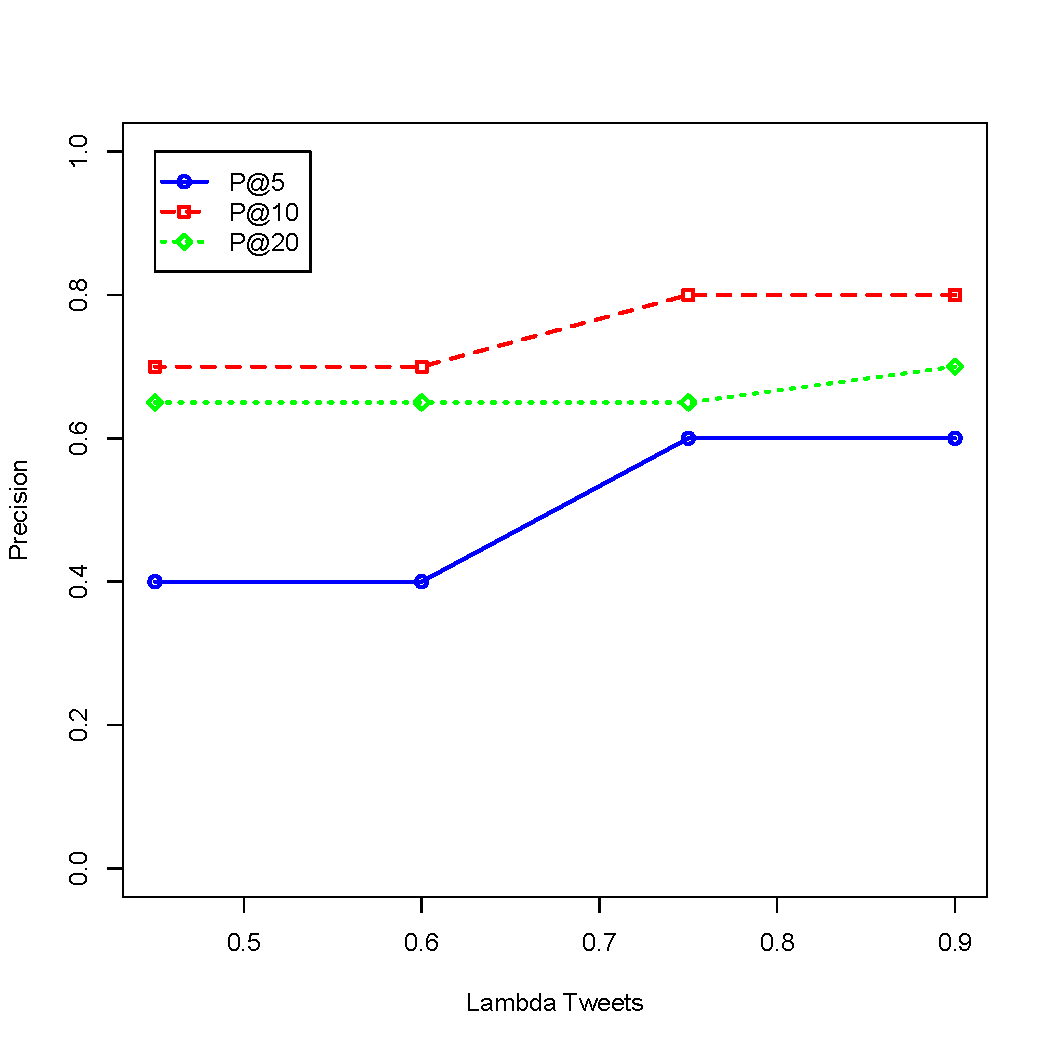
\includegraphics[scale=0.75]{Ki_Varying_LambdaTweets_UserResults}
  \caption[User recommendation results for user $K_{i}$ when varying $\lambda_{tweets}$]{User recommendation results for user $K_{i}$ when varying $\lambda_{tweets}$. The value of $\lambda_{users}$ is held constant at 0.7.}
  \label{fig:UsersForVaryingLambdaTweets}
\end{figure}
\begin{figure}
  \centering
  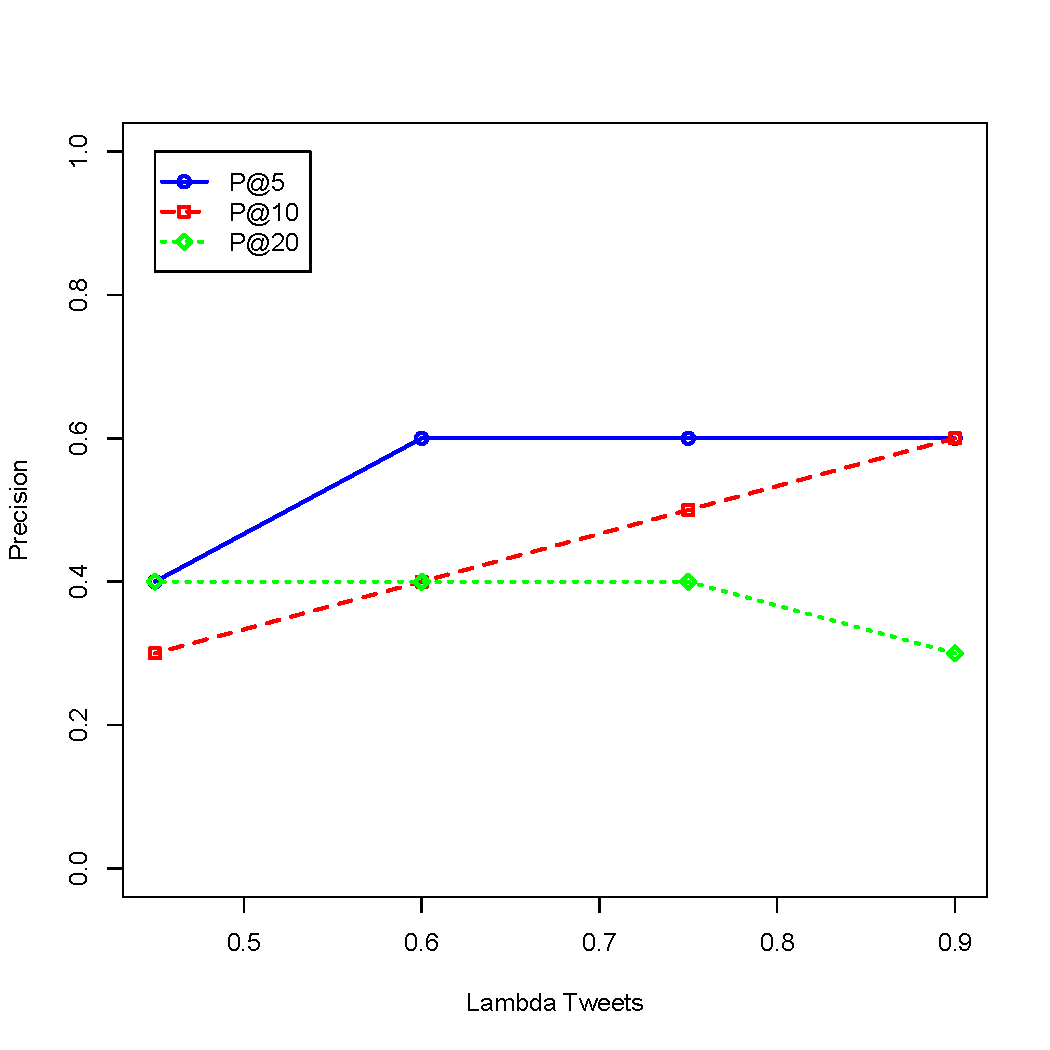
\includegraphics[scale=0.75]{Ki_Varying_LambdaTweets_TweetResults}
  \caption[Tweet recommendation results for user $K_{i}$ when varying $\lambda_{tweets}$]{Tweet recommendation results for user $K_{i}$ when varying $\lambda_{tweets}$. The value of $\lambda_{users}$ is held constant at 0.7.}
  \label{fig:TweetsForVaryingLambdaTweets}
\end{figure}


Figure~\ref{fig:UsersForVaryingLambdaUsers} shows the results of the user recommendations for user $K_{i}$ when varying the $\lambda_{users}$ parameter, while Figure~\ref{fig:TweetsForVaryingLambdaUsers} shows the results of the tweet recommendations for user $K_{i}$ when varying the $\lambda_{users}$ parameter. Both of these graphs confirm that a value of lambda tweets too close to 1 will provide terrible results. Because the initial scores for the users are so good, it does not particularly matter how close to 0 the value of lambda users gets.

\begin{figure}
  \centering
  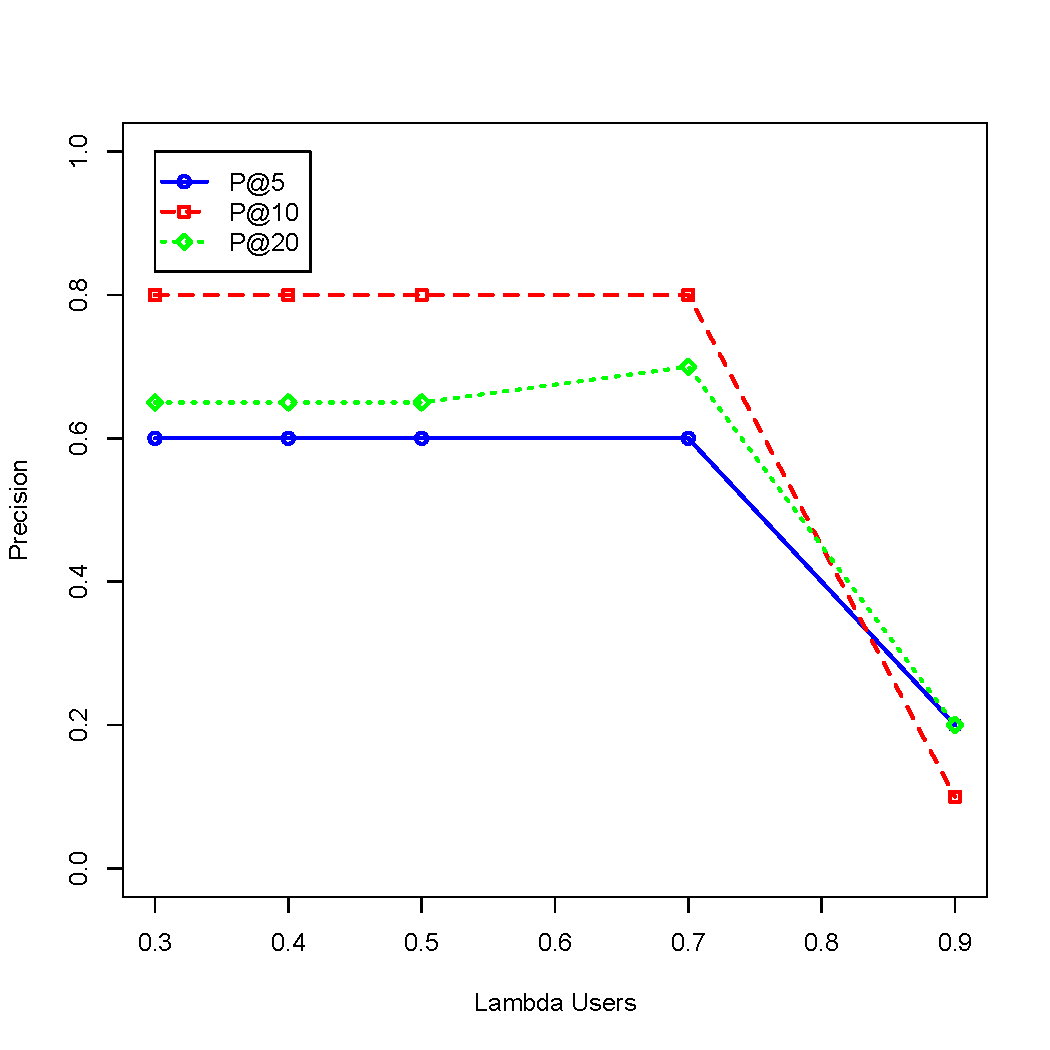
\includegraphics[scale=0.75]{Ki_Varying_LambdaUsers_UserResults}
  \caption[User recommendation results for user $K_{i}$ when varying $\lambda_{users}$]{User recommendation results for user $K_{i}$ when varying $\lambda_{users}$. The value of $\lambda_{tweets}$ is held constant at 0.9.}
  \label{fig:UsersForVaryingLambdaUsers}
\end{figure}
\begin{figure}
  \centering
  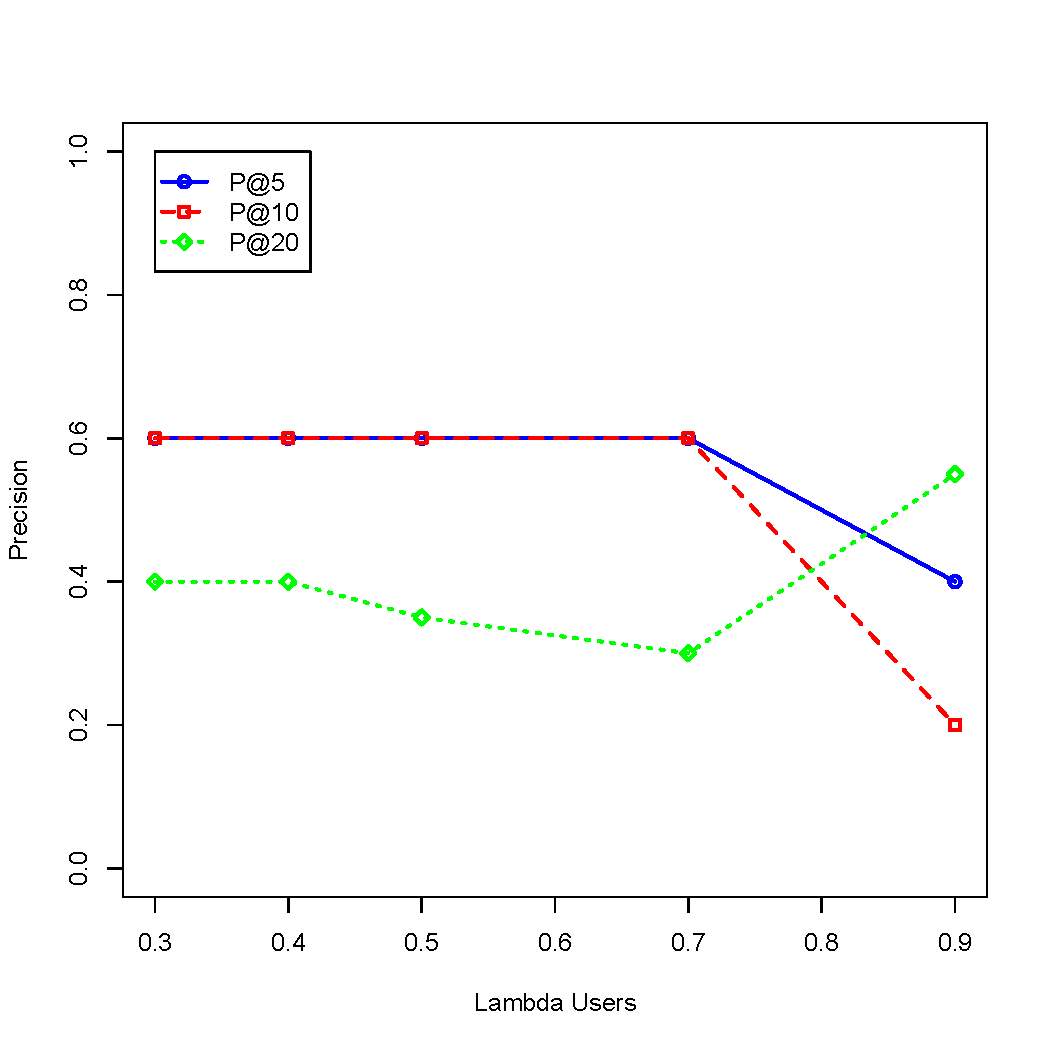
\includegraphics[scale=0.75]{Ki_Varying_LambdaUsers_TweetResults}
  \caption[Tweet recommendation results for user $K_{i}$ when varying $\lambda_{users}$]{Tweet recommendation results for user $K_{i}$ when varying $\lambda_{users}$. The value of $\lambda_{tweets}$ is held constant at 0.9.}
  \label{fig:TweetsForVaryingLambdaUsers}
\end{figure}


Another test was undertaken for user $K_{j}$, which was to hold $\lambda_{users}$ constant at 0.9 while varying the tweets parameter. Though not many data points were collected, it does still suggest that keeping the value of the $\lambda_{tweets}$ parameter closer to 1 is preferable. The graph for the user recommendation results on this data is shown in Figure~\ref{fig:KjUsersForVaryingLambdaTweets}, while the graph for the user recommendation results on this data is shown in Figure~\ref{fig:KjTweetsForVaryingLambdaTweets}. The results are not as good as when the value of $\lambda_{users}$ is closer to the optimal values revealed in the other experiments in this section.

\begin{figure}
  \centering
  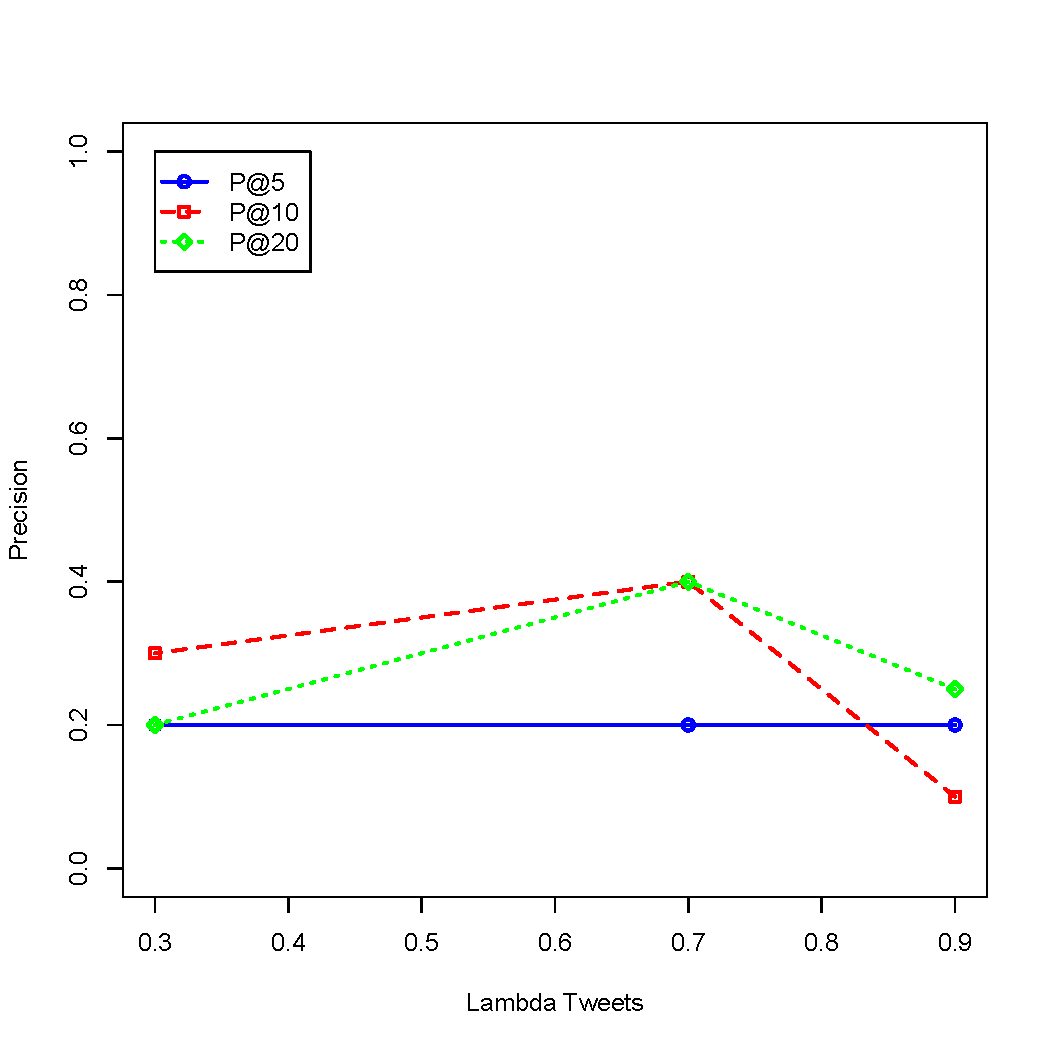
\includegraphics[scale=0.75]{Kj_Varying_LambdaTweets_UserResults}
  \caption[User recommendation results for user $K_{j}$ when varying $\lambda_{tweets}$]{User recommendation results for user $K_{j}$ when varying $\lambda_{tweets}$. The value of $\lambda_{users}$ is held constant at 0.9.}
  \label{fig:KjUsersForVaryingLambdaTweets}
\end{figure}
\begin{figure}
  \centering
  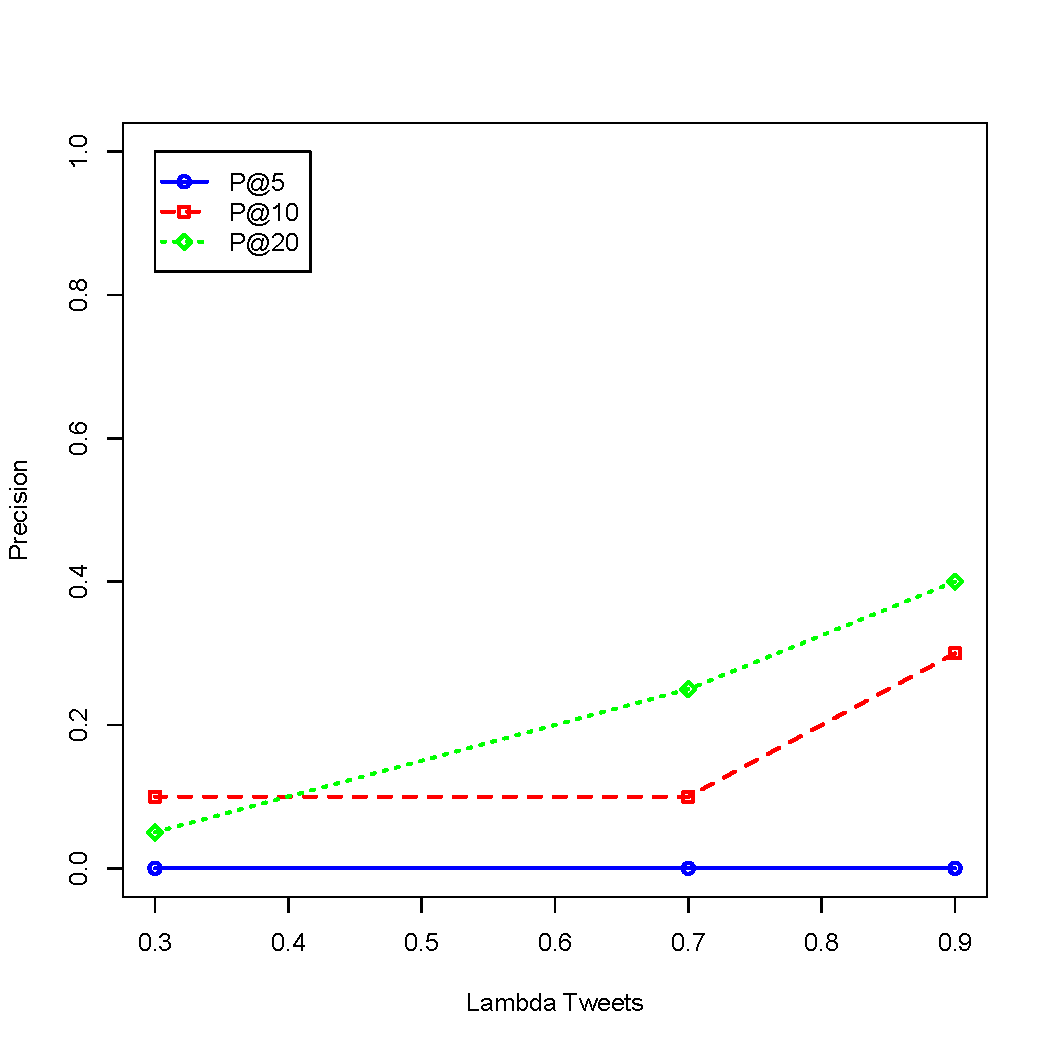
\includegraphics[scale=0.75]{Kj_Varying_LambdaTweets_TweetResults}
  \caption[Tweet recommendation results for user $K_{j}$ when varying $\lambda_{tweets}$]{Tweet recommendation results for user $K_{j}$ when varying $\lambda_{tweets}$. The value of $\lambda_{users}$ is held constant at 0.9.}
  \label{fig:KjTweetsForVaryingLambdaTweets}
\end{figure}

A final experiment on the lambda parameters was undertaken which moved both $\lambda$ parameters to 1, thereby removing much of the impact of the initial scores. The results for this configuration were terrible, with the precision for both tweets and users being 0.2, the average scores being between 2.5 and 2.75, and no scores of 5 for any of the user recommendations. The results for this experiment are included as part of the experiments on varying the types of edge included in the algorithm described in Section~\ref{sec:VaryingEdgeTypes}.



\subsection{Varying Edge Types Included}
\label{sec:VaryingEdgeTypes}

As was mentioned in Chapter 4, the algorithm was slow to run due to database access times. This made it difficult to experiment with removing edge types because with twelve different edge types there were a large number of possible combinations that could have been removed. Instead, the experiments focused on removing the edge types that seemed like they might be less valuable.

Recall the edge types from Table~\ref{tab:EdgeTypes}. The retweet, mention, and at-reply edges connect the user who was retweeted, mentioned, or at-replied to with the tweet that retweeted, mentioned, or at-replied to them. The logic behind this was previously discussed, but the link is a tenuous one and thus these are prime candidates for removal to see the effect on the results. Note that the other five retweet, mention, and at-reply edges remained in place.

There were 292,475 edges of these types, which is a very small amount in the context of 120 million total edges, and as can be seen from the results from removing these edges shown in Table~\ref{tab:Remove369}, removing these edges had very little impact on the overall quality of the results when compared with the baseline results already presented, and what little impact there was tended to be negative. This experiment was done for user $K_{i}$ only and it is difficult to draw too many conclusions from such a small smaple size, but since the edges do not seem to be particularly valuable they could perhaps be removed from the graph entirely in order to speed up the algorithm.


\begin{table}
\centering
\begin{tabular}{l|p{2cm}|p{2cm}|p{2cm}|p{2cm}}
{\bf Metric} & {\bf $K_{i}$ Base Config. User Scores} & {\bf $K_{j}$ User Scores} & {\bf $K_{i}$ Base Config. Tweet Scores} & {\bf $K_{j}$ Tweet Scores} \\ \hline
P@5   & 0.6 & 0.6 & 0.6 & 0.4 \\ \hline
P@10 & 0.8 & 0.8 & 0.6 & 0.5 \\ \hline
P@15 & 0.733 & 0.666 & 0.4 & 0.333 \\ \hline
P@20 & 0.7 & 0.65 & 0.3 & 0.25 \\ \hline

Avg. Score @5   & 3.0 & 3.0 & 3.4 & 3.4 \\ \hline
Avg. Score @10 & 3.7 & 3.7 & 3.3 & 3.4 \\ \hline
Avg. Score @15 & 3.733 & 3.6 & 2.933 & 2.866 \\ \hline
Avg. Score @20 & 3.65 & 3.6 & 2.9 & 2.7 \\ \hline

\% 5s@5    & 20\% & 20\% & - & - \\ \hline
\% 5s@10  & 30\% & 30\% & - & - \\ \hline
\% 5s@15  & 26.6\% & 26.6\% & - & - \\ \hline
\% 5s@20  & 20\% & 20\% & - & - \\

\end{tabular}
\caption{The tweet score and user score results for user $K_{i}$ when removing the simple retweet, mention, and @reply edges.}
\label{tab:Remove369}
\end{table}



The results from removing one or both of the types of content edges were only slightly clearer, though the impact improved the results rather than hurting them. Two basic experiments were run: one that removed all content edges (cf Table~\ref{tab:RemoveContent}) and one that removed only the hashtag edges (cf Table~\ref{tab:RemoveHashtags}). There were a lot of the content edges: about 42 million hashtag edges and about 38 million entity-based edges. It was surprising, then, when removing them had such a small effect. Comparing the results in Table~\ref{tab:RemoveContent} with the baseline results already presented shows very little difference. As with the other experiment with removing edges, this experiment was only run for user $K_{i}$.

\begin{table}
\centering
\begin{tabular}{l|p{2.2cm}|p{2.2cm}|p{2.2cm}|p{2.2cm}}
{\bf Metric} & {\bf $K_{i}$ Base User Scores} & {\bf $K_{i}$ User Scores} & {\bf $K_{i}$ Base Tweet Scores} & {\bf $K_{i}$ Tweet Scores} \\ \hline
P@5   & 0.6 & 0.6 & 0.6 & 0.6 \\ \hline
P@10 & 0.8 & 0.8 & 0.6 & 0.6 \\ \hline
P@15 & 0.733 & 0.866 & 0.4 & 0.466 \\ \hline
P@20 & 0.7 & 0.8 & 0.3 & 0.45 \\ \hline

Avg. Score @5   & 3.0 & 2.8 & 3.4 & 3.6 \\ \hline
Avg. Score @10 & 3.7 & 3.5 & 3.3 & 3.7 \\ \hline
Avg. Score @15 & 3.733 & 3.8 & 2.933 & 3.333 \\ \hline
Avg. Score @20 & 3.65 & 3.7 & 2.9 & 3.25 \\ \hline

\% 5s@5    & 20\% & 0\% & - & - \\ \hline
\% 5s@10  & 30\% & 10\% & - & - \\ \hline
\% 5s@15  & 26.6\% & 20\% & - & - \\ \hline
\% 5s@20  & 20\% & 20\% & - & - \\

\end{tabular}
\caption{Results for user $K_{i}$ from removing all content edges, as compared with the base configuration}
\label{tab:RemoveContent}
\end{table}


\begin{table}
\centering
\begin{tabular}{l|p{2.2cm}|p{2.2cm}|p{2.2cm}|p{2.2cm}}
{\bf Metric} & {\bf $K_{i}$ Base User Scores} & {\bf $K_{i}$ User Scores} & {\bf $K_{i}$ Base Tweet Scores} & {\bf $K_{i}$ Tweet Scores} \\ \hline
P@5   & 0.6 & 0.6 & 0.6 & 0.6 \\ \hline
P@10 & 0.8 & 0.8 & 0.6 & 0.7 \\ \hline
P@15 & 0.733 & 0.733 & 0.4 & 0.533 \\ \hline
P@20 & 0.7 & 0.7 & 0.3 & 0.45 \\ \hline

Avg. Score @5   & 3.0 & 3.0 & 3.4 & 3.4 \\ \hline
Avg. Score @10 & 3.7 & 3.7 & 3.3 & 3.7 \\ \hline
Avg. Score @15 & 3.733 & 3.666 & 2.933 & 3.4 \\ \hline
Avg. Score @20 & 3.65 & 3.65 & 2.9 & 3.25 \\ \hline

\% 5s@5    & 20\% & 20\% & - & - \\ \hline
\% 5s@10  & 30\% & 30\% & - & - \\ \hline
\% 5s@15  & 26.6\% & 26.6\% & - & - \\ \hline
\% 5s@20  & 20\% & 20\% & - & - \\

\end{tabular}
\caption{Results for user $K_{i}$ from removing the hashtags edges only, as compared with the base configuration}
\label{tab:RemoveHashtags}
\end{table}


In order to attempt to isolate the effect of removing the edges from the effect of the initial scores, the removal of the content edges was also performed with both $\lambda$ parameters set to 1. The results for this are particularly interesting in that the results for the quality of the user recommendations were much lower than the default configuration and even lower than with the content edges in place, while the tweet scores improved greatly. This result is shown in Table~\ref{tab:RemoveContentLambdasAt1}, which compares the results of the user and tweet recommendations for user $K_{i}$ with the content edges in place but the $\lambda$ parameters set to 1 and the recommendations with the $\lambda$ parameters set to 1 but the content edges removed. As with all of the experimental variations described here, the sample size is too small to draw any firm conclusions, but it still suggests an interesting avenue for further exploration in the future.


\begin{table}
\centering
\begin{tabular}{l|p{2cm}|p{2cm}|p{2cm}|p{2cm}}
{\bf Metric} & {\bf $\lambda_{t,u}=1$ Base User Scores} & {\bf User Scores} & {\bf $\lambda_{t,u}=1$ Base Tweet Scores} & {\bf Tweet Scores} \\ \hline
P@5   & 0.0 & 0.2 & 0.2 & 0.6 \\ \hline
P@10 & 0.2 & 0.1 & 0.2 & 0.7 \\ \hline
P@15 & 0.2 & 0.133 & 0.2 & 0.533 \\ \hline
P@20 & 0.2 & 0.1 & 0.2 & 0.45 \\ \hline

Avg. Score @5   & 2.4 & 2.4 & 2.8 & 3.8 \\ \hline
Avg. Score @10 & 2.7 & 2.3 & 2.8 & 3.9 \\ \hline
Avg. Score @15 & 2.8 & 2.2 & 2.733 & 3.4 \\ \hline
Avg. Score @20 & 2.6 & 2.05 & 2.7 & 3.15 \\ \hline

\% 5s@5    & 0\% & 0\% & - & - \\ \hline
\% 5s@10  & 0\% & 0\% & - & - \\ \hline
\% 5s@15  & 0\% & 0\% & - & - \\ \hline
\% 5s@20  & 0\% & 0\% & - & - \\

\end{tabular}
\caption{The tweet score and user score results for user $K_{i}$ when removing the content edges with the $\lambda$ parameters set to 1}
\label{tab:RemoveContentLambdasAt1}
\end{table}

One final test on removing edges combined the two main edge types that were experimented on by removing the retweet, mention, and at-reply edges in addition to the two types of content edges. Again, the $\lambda$ parameters were set to 1 in an attempt to remove the impact of the initial scores on the outcome. For the user recommendations these results were slightly better than those from removing only the content edges, while for the tweet recommendations they were more mixed, with the top 10 showing worse results and the rest of the top 20 showing improved results. The usual caveats about small sample size apply here as well, of course.

\begin{table}
\centering
\begin{tabular}{l|p{2cm}|p{2cm}|p{2cm}|p{2cm}}
{\bf Metric} & {\bf $\lambda_{t,u}=1$ Base User Scores} & {\bf User Scores} & {\bf $\lambda_{t,u}=1$ Base Tweet Scores} & {\bf Tweet Scores} \\ \hline
P@5   & 0.0 & 0.4 & 0.2 & 0.6 \\ \hline
P@10 & 0.2 & 0.2 & 0.2 & 0.5 \\ \hline
P@15 & 0.2 & 0.2 & 0.2 & 0.666 \\ \hline
P@20 & 0.2 & 0.15 & 0.2 & 0.75 \\ \hline

Avg. Score @5   & 2.4 & 3.2 & 2.8 & 3.8 \\ \hline
Avg. Score @10 & 2.7 & 2.7 & 2.8 & 3.5 \\ \hline
Avg. Score @15 & 2.8 & 2.666 & 2.733 & 3.666 \\ \hline
Avg. Score @20 & 2.6 & 2.15 & 2.7 & 3.75 \\ \hline

\% 5s@5    & 0\% & 0\% & - & - \\ \hline
\% 5s@10  & 0\% & 0\% & - & - \\ \hline
\% 5s@15  & 0\% & 0\% & - & - \\ \hline
\% 5s@20  & 0\% & 0\% & - & - \\

\end{tabular}
\caption{The tweet score and user score results for user $K_{i}$ when removing the content edges and the simple retweet, mention, and @reply edges with the $\lambda$ parameters set to 1.}
\label{tab:RemoveContentAnd369LambdasAt1}
\end{table}


\subsection{Varying Edge Weights}

The slowness of running the algorithm made experimentation on edge weights particularly difficult because with so many different edges and possible weightings for them a rigorous experiment would require far more time than was available. As such, the experiments which were done were based largely on intuition and were small in number, with only four different weightings being explored.

The experiments done here were performed on user $K_{j}$, with directionality per the default, though authorship edges were bi-directional. Table~\ref{tab:EdgeWeightsUsed} shows the weights that were used for each edge type in each experiment. Table~\ref{tab:WeightsTestsUsers} shows the results for each experiment on the user recommendations and Table~\ref{tab:WeightsTestsTweets} shows the results for each experiment on the tweet recommendations. Note that the edges corresponding to basic retweets, mentions, and at replies were not included for any of these experiments, and thus no weights are listed for these edge types.

The methodology used was to sum the total weight of all edges emanating from a vertex, and the chance of taking a particular edge was just the weight of that edge's type divided by the total weight of all edges. So if a particular vertex had two edges with a weight of 2 each and one edge with a weight of  0.5 then the total weight would be 4.5, so the chance of going to each of the edges with weight 2 would be $2 \div 4.5 = 0.44$ and the chance of going to the edge with weight 0.5 would be $0.5 \div 4.5 = 0.11$.


\begin{table}
\centering
\begin{tabular}{l|p{1.5cm}|p{1.5cm}|p{1.5cm}|p{1.5cm}}
{\bf Edge Type} & {\bf Test 1 Weight} & {\bf Test 2 Weight} & {\bf Test 3 Weight} & {\bf Test 4 Weight} \\ \hline
Authorship & 2 & 2 & 2 & 4 \\ \hline
Follower & 1.25 & 1.25 & 1.25 & 1.5 \\ \hline
Retweet Followees & 2 & 3 & 3 & 3 \\ \hline
Retweet Followers & 0.75 & 1.25 & 1.25 & 1.25 \\ \hline
Mention Followees & 2 & 2 & 2 & 1.5 \\ \hline
Mention Followers & 0.75 & 1 & 1 & 1 \\ \hline
@reply Content & 0.5 & 0.5 & 0.25 & 0.5 \\ \hline
Hashtag & 1 & 1 & 3.5 & 1 \\ \hline
Content & 1 & 1 & 1.5 & 1 \\
\end{tabular}
\caption{Edge weights used for each experiment }
\label{tab:EdgeWeightsUsed}
\end{table}

\begin{table}
\centering
\begin{tabular}{l|p{1.5cm}|p{1.5cm}|p{1.5cm}|p{1.5cm}|p{1.5cm}}
{\bf Metric} & {\bf $K_{j}$ Base User Scores} & {\bf Test 1 User Scores} & {\bf Test 2 User Scores} & {\bf Test 3 User Scores} & {\bf Test 4 User Scores} \\ \hline
P@5   & 0.6 & 0.6 & 0.6 & 0.6 & 0.6 \\ \hline
P@10 & 0.6 & 0.6 & 0.6 & 0.6 & 0.6 \\ \hline
P@15 & 0.6 & 0.533 & 0.6 & 0.6 & 0.6 \\ \hline
P@20 & 0.55 & 0.6 & 0.65 & 0.6 & 0.6 \\ \hline

Avg. Score @5   & 3.4 & 3.4 & 3.4 & 3.4 & 3.4 \\ \hline
Avg. Score @10 & 3.5 & 3.7 & 3.7 & 3.7 & 3.7 \\ \hline
Avg. Score @15 & 3.6 & 3.4 & 3.666 & 3.666 & 3.666 \\ \hline
Avg. Score @20 & 3.35 & 3.5 & 3.65 & 3.65 & 3.65 \\ \hline

\% 5s@5    & 20\% & 40\% & 40\% & 40\% & 40\% \\ \hline
\% 5s@10  & 40\% & 40\% & 40\% & 40\% & 40\% \\ \hline
\% 5s@15  & 33.3\% & 33.3\% & 40\% & 40\% & 40\% \\ \hline
\% 5s@20  & 25\% & 30\% & 30\% & 30\% & 30\% \\
\end{tabular}
\caption{Results of the user recommendations for user $K_{j}$ when varying the weights of the edges}
\label{tab:WeightsTestsUsers}
\end{table}


\begin{table}
\centering
\begin{tabular}{l|p{1.5cm}|p{1.5cm}|p{1.5cm}|p{1.5cm}|p{1.5cm}}
{\bf Metric} & {\bf $K_{j}$ Base Tweet Scores} & {\bf Test 1 Tweet Scores} & {\bf Test 2 Tweet Scores} & {\bf Test 3 Tweet Scores} & {\bf Test 4 Tweet Scores} \\ \hline
P@5   & 0.0 & 0.4 & 0.4 & 0.4 & 0.4 \\ \hline
P@10 & 0.2 & 0.3 & 0.4 & 0.4 & 0.4 \\ \hline
P@15 & 0.4 & 0.4 & 0.4 & 0.4 & 0.4 \\ \hline
P@20 & 0.4 & 0.35 & 0.35 & 0.35 & 0.35 \\ \hline

Avg. Score @5   & 2.8 & 3.4 & 3.4 & 3.4 & 3.4 \\ \hline
Avg. Score @10 & 3.1 & 3.3 & 3.4 & 3.4 & 3.4 \\ \hline
Avg. Score @15 & 3.266 & 3.4 & 3.4 & 3.4 & 3.4 \\ \hline
Avg. Score @20 & 3.3 & 3.3 & 3.3 & 3.3 & 3.4 \\
\end{tabular}
\caption{Results of the tweet recommendations for user $K_{j}$ when varying the weights of the edges}
\label{tab:WeightsTestsTweets}
\end{table}

One very clear result from the experiments is that none of them gave results which were particularly distinct, though the weights in the fourth experiment were perhaps slightly better. The most likely reason for this is that the values for the weights of the various edges were not very distinct between the different experiments. Instead, they were based on a few assumptions, such as that retweets, followers, and authorship are very important. Existing research and some of the other experiments support these intuitions, but the experiments run here neither proved nor disproved them.


\subsection{Varying Edge Directionality}
\label{sec:VaryingEdgeDirectionality}

The directionality of the edges when producing the baseline results described in Section~\ref{sec:BaselineResults} followed the description in Table~\ref{tab:EdgeTypes}. As shown in that section, this directionality produced generally good recommendations for both users and tweets.

One obvious variation on these baseline results is to remove edge directionality altogether and assume that each edge type has an influence in both directions. For at least some of the edge types, this makes perfect sense. Consider the authorship edge, for example. It certainly makes sense that if a particular tweet received a high score because of something it was connected to then that score should be passed along to the author of the tweet. Similarly, a highly scoring user should obviously transfer some of that high score along to the tweets that they author.

Running the algorithm with all edge types being bi-directional was one of the first experiments that was run for user $U$. The results from doing this were very clearly terrible. The tweets were dominated by one or two users and the tweets of those users were political in nature and diametrically opposed to the political views of the distinguished user. On the scale used for the user study, all of these would have ranked as a 2 had user $U$ been part of the user study.

The reason for this was that the user who produced the tweets followed over 40,000 people, and today follows more than 80,000 people. Clearly this user does not interact with or even read all of the tweets from these 40,000 people, but the algorithm cannot take that into account. So because this user tweeted frequently and followed so many people, their tweets were highly scored by the system with bi-directional edges because each of their 19 tweets was connected to thousands of users whose scores all contributed to high scores for these tweets.

This result demonstrates that for the edges based on the network state it does not makes sense to vary the directionality of the edges, either by reversing them or by making them bi-directional. Take follower edges for example: clearly there is not an influence by a user on the tweets of someone they follow. This was the biggest issue in the experiment done with no directionality at all---it assumed influence where there was none and came up with correspondingly terrible results.

Eliminating the network edges from consideration then leaves only the two content-based edges and the authorship edge as candidates for changing directionality. With these edges it is not clear that any one direction should be the one that has the influence; for instance, it could make sense that all tweets on a given subject should provide their scores to a user or that a highly scoring user should provide an impact on all tweets mentioning subjects of a similar subject. Similarly, leaving these as bi-directional as in the default configuration also makes sense.


\begin{table}
\centering
\begin{tabular}{l|p{2.2cm}|p{2.2cm}|p{2.2cm}|p{2.2cm}}
{\bf Metric} & {\bf $K_{i}$ Base User Scores} & {\bf $K_{i}$ User Scores} & {\bf $K_{i}$ Base Tweet Scores} & {\bf $K_{i}$ Tweet Scores} \\ \hline
P@5   & 0.6 & 0.6 & 0.6 & 0.6 \\ \hline
P@10 & 0.8 & 0.8 & 0.6 & 0.7 \\ \hline
P@15 & 0.733 & 0.866 & 0.4 & 0.533 \\ \hline
P@20 & 0.7 & 0.75 & 0.3 & 0.45 \\ \hline

Avg. Score @5   & 3.0 & 3.0 & 3.4 & 3.6 \\ \hline
Avg. Score @10 & 3.7 & 3.6 & 3.3 & 3.8 \\ \hline
Avg. Score @15 & 3.733 & 3.866 & 2.933 & 3.4 \\ \hline
Avg. Score @20 & 3.65 & 3.7 & 2.9 & 3.25 \\ \hline

\% 5s@5    & 20\% & 20\% & - & - \\ \hline
\% 5s@10  & 30\% & 20\% & - & - \\ \hline
\% 5s@15  & 26.6\% & 26.6\% & - & - \\ \hline
\% 5s@20  & 20\% & 20\% & - & - \\

\end{tabular}
\caption{Results for user $K_{i}$ when content edges are directed from tweet to user}
\label{tab:ContentTweetToUser}
\end{table}


\begin{table}
\centering
\begin{tabular}{l|p{2.2cm}|p{2.2cm}|p{2.2cm}|p{2.2cm}}
{\bf Metric} & {\bf $K_{i}$ Base User Scores} & {\bf $K_{i}$ User Scores} & {\bf $K_{i}$ Base Tweet Scores} & {\bf $K_{i}$ Tweet Scores} \\ \hline
P@5   & 0.6 & 0.6 & 0.6 & 0.8 \\ \hline
P@10 & 0.8 & 0.6 & 0.6 & 0.6 \\ \hline
P@15 & 0.733 & 0.733 & 0.4 & 0.466 \\ \hline
P@20 & 0.7 & 0.7 & 0.3 & 0.35 \\ \hline

Avg. Score @5   & 3.0 & 3.0 & 3.4 & 4.4 \\ \hline
Avg. Score @10 & 3.7 & 3.2 & 3.3 & 3.6 \\ \hline
Avg. Score @15 & 3.733 & 3.6 & 2.933 & 3.266 \\ \hline
Avg. Score @20 & 3.65 & 3.6 & 2.9 & 2.9 \\ \hline

\% 5s@5    & 20\% & 20\% & - & - \\ \hline
\% 5s@10  & 30\% & 10\% & - & - \\ \hline
\% 5s@15  & 26.6\% & 20\% & - & - \\ \hline
\% 5s@20  & 20\% & 20\% & - & - \\
\end{tabular}
\caption{Results for user $K_{i}$ when content edges are directed from user to tweet}
\label{tab:ContentUserToTweet}
\end{table}

Both directions for the content edges yield improved results for the tweet recommendations, which is quite a surprising result. Directing the content edges from tweet to user yields slightly better user recommendations, though the recommendations are quite good in both cases. Table~\ref{tab:ContentTweetToUser} shows the results when content edges are directed from tweet vertices to user vertices and Table~\ref{tab:ContentUserToTweet} shows the results when the content edges go in the other direction.


Experiments were also done with the authorship edge. By default this edge was directed from the user to the tweet, but as was previously discussed this could certainly have been bi-directional. The results shown in Table~\ref{tab:BiDirectionalAuthorKi} are from running the algorithm for user $K_{i}$ with all the standard edges and directions but with the authorship edge being bi-directional. Table~\ref{tab:BiDirectionalAuthorKj}, meanwhile, shows the same experiment for user $K_{j}$. The results for this configuration show that changing the direction of these 500,000 edges has almost no effect.

\begin{table}
\centering
\begin{tabular}{l|p{2.2cm}|p{2.2cm}|p{2.2cm}|p{2.2cm}}
{\bf Metric} & {\bf $K_{i}$ Base User Scores} & {\bf $K_{i}$ User Scores} & {\bf $K_{i}$ Base Tweet Scores} & {\bf $K_{i}$ Tweet Scores} \\ \hline
P@5   & 0.6 & 0.6 & 0.6 & 0.6 \\ \hline
P@10 & 0.8 & 0.8 & 0.6 & 0.5 \\ \hline
P@15 & 0.733 & 0.733 & 0.4 & 0.4 \\ \hline
P@20 & 0.7 & 0.65 & 0.3 & 0.4 \\ \hline

Avg. Score @5   & 3.0 & 3.0 & 3.4 & 3.6 \\ \hline
Avg. Score @10 & 3.7 & 3.7 & 3.3 & 3.3 \\ \hline
Avg. Score @15 & 3.733 & 3.733 & 2.933 & 3.0 \\ \hline
Avg. Score @20 & 3.65 & 3.6 & 2.9 & 3.1 \\ \hline

\% 5s@5    & 20\% & 20\% & - & - \\ \hline
\% 5s@10  & 30\% & 30\% & - & - \\ \hline
\% 5s@15  & 26.6\% & 26.6\% & - & - \\ \hline
\% 5s@20  & 20\% & 20\% & - & - \\
\end{tabular}
\caption{Results for user $K_{i}$ when the authorship edge is bi-directional.}
\label{tab:BiDirectionalAuthorKi}
\end{table}



\begin{table}
\centering
\begin{tabular}{l|p{2.2cm}|p{2.2cm}|p{2.2cm}|p{2.2cm}}
{\bf Metric} & {\bf $K_{j}$ Base User Scores} & {\bf $K_{j}$ User Scores} & {\bf $K_{j}$ Base Tweet Scores} & {\bf $K_{j}$ Tweet Scores} \\ \hline
P@5   & 0.6 & 0.6 & 0.0 & 0.0 \\ \hline
P@10 & 0.6 & 0.6 & 0.2 & 0.2 \\ \hline
P@15 & 0.6 & 0.6 & 0.4 & 0.266 \\ \hline
P@20 & 0.55 & 0.6 & 0.4 & 0.3 \\ \hline

Avg. Score @5   & 3.4 & 3.4 & 2.8 & 2.8 \\ \hline
Avg. Score @10 & 3.5 & 3.7 & 3.1 & 3.0 \\ \hline
Avg. Score @15 & 3.6 & 3.6 & 3.266 & 3.133 \\ \hline
Avg. Score @20 & 3.35 & 3.5 & 3.3 & 3.2 \\ \hline

\% 5s@5    & 20\% & 40\% & - & - \\ \hline
\% 5s@10  & 40\% & 40\% & - & - \\ \hline
\% 5s@15  & 33.3\% & 33\% & - & - \\ \hline
\% 5s@20  & 25\% & 30\% & - & - \\

\end{tabular}
\caption{Results for user $K_{j}$ when the authorship edge is bi-directional.}
\label{tab:BiDirectionalAuthorKj}
\end{table}



\subsection{Combined Configuration}
\label{sec:CombinedConfiguration}

Most of the experiments showed very mixed results for individual variations, with most of the experiments making very little difference on the final outcome. The values for the $\lambda$ parameters were fairly clear, but changing the included edges and the edge directions had little effect. Still, one thing that has not been explored thus far is a combination of some these different features. The results in this section combine some of the past experiments into a combined configuration in hopes that the combination will produce better results than the generally middling results of the previous experiments. Unfortunately, the results are generally comparable to those of the baseline configuration, though perhaps a more robust experiment which studied more users would reveal more clear-cut results.

Table~\ref{tab:BiAuthorNo369Ki} shows the results for user $K_{i}$ with the authorship edge being bi-directional and the simple retweet, mention, and at-reply edges being removed. As with many of the other experimental variations the results differ only slightly from the baseline results, and only one or two tweets and users are different. Table~\ref{tab:BiAuthorNo369Kj} shows the results of the same experiment for $K_{j}$, which shows slightly better results. The tweet recommendations for user $K_{j}$ do show quite a bit of improvement early in the recommendations list, though this is due in no small part to the fact that the baseline tweet results for this user were poor to begin with.

By default, the algorithm ignores the duplicate edges of the same type linking a user and a tweet that exist in the graph. As an additional experiment on user $K_{i}$, the experiment shown was repeated with the duplicate edges in the graph being left in. The results for this were identical to the results when leaving these edges out. This surprising result suggests a possible way to speed up the algorithm, since more than 10 million of the edges are duplicates.


\begin{table}
\centering
\begin{tabular}{l|p{2.2cm}|p{2.2cm}|p{2.2cm}|p{2.2cm}}
{\bf Metric} & {\bf $K_{i}$ Base User Scores} & {\bf $K_{i}$ User Scores} & {\bf $K_{i}$ Base Tweet Scores} & {\bf $K_{i}$ Tweet Scores} \\ \hline
P@5   & 0.6 & 0.6 & 0.6 & 0.4 \\ \hline
P@10 & 0.8 & 0.8 & 0.6 & 0.4 \\ \hline
P@15 & 0.733 & 0.666 & 0.4 & 0.4 \\ \hline
P@20 & 0.7 & 0.6 & 0.3 & 0.3 \\ \hline

Avg. Score @5   & 3.0 & 3.0 & 3.4 & 3.4 \\ \hline
Avg. Score @10 & 3.7 & 3.7 & 3.3 & 3.2 \\ \hline
Avg. Score @15 & 3.733 & 3.6 & 2.933 & 3.066 \\ \hline
Avg. Score @20 & 3.65 & 3.55 & 2.9 & 2.8 \\ \hline

\% 5s@5    & 20\% & 20\% & - & - \\ \hline
\% 5s@10  & 30\% & 30\% & - & - \\ \hline
\% 5s@15  & 26.6\% & 26.6\% & - & - \\ \hline
\% 5s@20  & 20\% & 20\% & - & - \\
\end{tabular}
\caption{Results for user $K_{i}$ with the authorship edge being bi-directional and the retweet, mention, and @reply edges not included.}
\label{tab:BiAuthorNo369Ki}
\end{table}


\begin{table}
\centering
\begin{tabular}{l|p{2.2cm}|p{2.2cm}|p{2.2cm}|p{2.2cm}}
{\bf Metric} & {\bf $K_{j}$ Base User Scores} & {\bf $K_{j}$ User Scores} & {\bf $K_{j}$ Base Tweet Scores} & {\bf $K_{j}$ Tweet Scores} \\ \hline
P@5   & 0.6 & 0.6 & 0.0 & 0.4 \\ \hline
P@10 & 0.6 & 0.6 & 0.2 & 0.4 \\ \hline
P@15 & 0.6 & 0.6 & 0.4 & 0.333 \\ \hline
P@20 & 0.55 & 0.65 & 0.4 & 0.4 \\ \hline

Avg. Score @5   & 3.4 & 3.4 & 2.8 & 3.4 \\ \hline
Avg. Score @10 & 3.5 & 3.7 & 3.1 & 3.5 \\ \hline
Avg. Score @15 & 3.6 & 3.6 & 3.266 & 3.266 \\ \hline
Avg. Score @20 & 3.35 & 3.65 & 3.3 & 3.35 \\ \hline

\% 5s@5    & 20\% & 40\% & - & - \\ \hline
\% 5s@10  & 40\% & 40\% & - & - \\ \hline
\% 5s@15  & 33.3\% & 33.3\% & - & - \\ \hline
\% 5s@20  & 25\% & 30\% & - & - \\

\end{tabular}
\caption{Results for user $K_{j}$ with the authorship edge being bi-directional and the retweet, mention, and @reply edges not included.}
\label{tab:BiAuthorNo369Kj}
\end{table}

One final experiment was run on $K_{j}$, similar to those on user $K_{i}$, but with the two content edge types not included. The results for this experiment are shown in Table~\ref{tab:BiAuthorNo369NoContent} and show that the early tweet recommendations were much improved over the baseline, while the user recommendations were about the same.


\begin{table}
\centering
\begin{tabular}{l|p{2.2cm}|p{2.2cm}|p{2.2cm}|p{2.2cm}}
{\bf Metric} & {\bf $K_{j}$ Base User Scores} & {\bf $K_{j}$ User Scores} & {\bf $K_{j}$ Base Tweet Scores} & {\bf $K_{j}$ Tweet Scores} \\ \hline
P@5   & 0.6 & 0.6 & 0.0 & 0.6 \\ \hline
P@10 & 0.6 & 0.5 & 0.2 & 0.5 \\ \hline
P@15 & 0.6 & 0.533 & 0.4 & 0.466 \\ \hline
P@20 & 0.55 & 0.5 & 0.4 & 0.4 \\ \hline

Avg. Score @5   & 3.4 & 3.4 & 2.8 & 3.6 \\ \hline
Avg. Score @10 & 3.5 & 3.3 & 3.1 & 3.5 \\ \hline
Avg. Score @15 & 3.6 & 3.4 & 3.266 & 3.466 \\ \hline
Avg. Score @20 & 3.35 & 3.3 & 3.3 & 3.4 \\ \hline

\% 5s@5    & 20\% & 40\% & - & - \\ \hline
\% 5s@10  & 40\% & 30\% & - & - \\ \hline
\% 5s@15  & 33.3\% & 26.6\% & - & - \\ \hline
\% 5s@20  & 25\% & 25\% & - & - \\

\end{tabular}
\caption{Results for user $K_{j}$ with the authorship edge being bi-directional and the retweet, mention, @reply, hashtag, and entity-based edges not included.}
\label{tab:BiAuthorNo369NoContent}
\end{table}



\section{Dataset Biases}

The results described in this chapter revealed some issues that come with selecting tweets to use for such a study that can end up having a major impact on the final results.

One drawback of the Twitter network is that particular communities are often over-represented, which can make it more difficult to find relevant content for people not in those communities. The tweet recommendations here show that effect quite clearly. User $U$ is a part of the Silicon Valley entrepreneurship community, which is very strongly represented on Twitter. Within the 500,000 tweets studied here that user's results were very good since there were a large number of tweets that would be interesting to someone from that community. But the trade-off is that there were far fewer tweets of interest available for the other users who were not part of that community.

Another bias in the Twitter dataset is that the subjects of the tweets can be overwhelmed by one particular event. The day that the tweets used here were collected happened to be World AIDS Day in 2009, resulting in a much higher level of discussion of things related to that than would normally be expected. This also had the effect of limiting the number of interesting tweets for someone who wasn't interested in content related to World AIDS Day.

Finally, because of limitations within the Twitter API and limitations of storing and collecting a large amount of data, the Twitter data used here only represents 20-30\% of tweets during the time period. This results in a lot of cases where a retweet is among the recommendations while the original tweet was never seen. The results could be improved if the repeated retweets of the same tweet were removed from the recommendations in favour of the original tweet.

All of these biases were noticeable in the results, though the impact was generally not a major one and the algorithm still produced excellent recommendations. It would be interesting and valuable to study the effect that these biases have on the results, such as by studying a larger number of tweets, a more complete dataset, or multiple different time periods.

That is far from the only work that remains to be done in this still very new research area, of course. While the results here are very promising, the experiments and methodologies suggest that plenty of improvements could be made and further experiments performed to improve the results described in this chapter. The final chapter will discuss some of the other future work that could be done to expand on and improve this project as well as providing concluding remarks on the project as a whole.







%5 -- Conclusions that can be drawn
\chapter{Conclusion}


\section{Enhancements and Future Work}

\subsection{Parallelization and Performance Improvement}

%TODO: find the stats of the server

Though the speed of the algorithm has not yet been described except in broad terms, it is extremely slow. This is not due to the inherent speed of the algorithm, but rather it owes to the fact that all of the data being used is stored in a series of databases on an external storage device and accessing that data is very slow.

The creation of the graph, for example, takes more than 24 hours due to the large number of lookups and insertions that must be done in order to connect more than 120 million edges. For example, for each tweet the followers of the author need to be looked up in order to determine the follower edge tweets, and then each of these edges must be inserted into the edges table in the database. The result is a slow process. Running the algorithm itself is much faster, but still on the order of hours rather than minutes or seconds. As with the speed of creating the graph, the slowness in running the algorithm is caused by the slowness of retrieving so much data from the hard disk.

It would be very reasonable to run many of the steps in parallel using an algorithm such as MapReduce and thus dramatically increase the speed of the entire process. If many different external storage devices are used, then the speed of initializing the user scores can be increased by running the initialization completely in parallel. The maximum limit of this process would be to have one external storage device for each user in the graph, allowing the initialization to be done in seconds.

The creation of the edges in the graph can also be run in parallel. In the existing algorithm, the creation of edges is done by iterating through each tweet and creating appropriate edges based on the type of tweet (mention, retweet, @reply), which entities and hashtags it contains, and who follows the author. It would be simple to duplicate the database information on multiple external storage devices and to look at multiple tweets in parallel.

And of course, the algorithm itself could also be run in parallel. Recall that the edges are ordered when they are retrieved for updating the scores for each side of the bipartite graph. The score contributions onto the other side are considered for each vertex, a process made easier by the fact that the edges are 


\subsection{Potential Enhancements}

%Not sure if this paragraph is worth keeping
One additional type of content edge that might be useful but which was not included in this project is a URL edge which connects tweets containing the same URL---in a shortened URL form using a service such as bit.ly, most likely---to the authors of those tweets. It wouldn't be feasible to expand all of the shortened URLs and to compare them that way, but since a given URL will always map to a particular shortened URL (at least for a period of several years) it is not necessary to expand them.



%now enable appendix numbering format and include any appendices
\appendix
%\include{appendix1}
%\include{appendix2}

%next line adds the Bibliography to the contents page
%\addcontentsline{toc}{chapter}{Bibliography}
%uncomment next line to change bibliography name to references
%\renewcommand{\bibname}{References}
\bibliography{bibliography}        %use bibliography.bib
\bibliographystyle{plain}  %use the plain bibliography style

\end{document}

